%% sample template file for a PhD Thesis
%% The default is with two sided setup:
\documentclass[%
%    oneside % uncomment for onesided layout
]{USN-PhD}

% --- Bibliography setup ---
%%% default is the "ieee" style
\usepackage[style=ieee, sorting=none]{biblatex}
%%% If you want to use "author-year" style
%%% where `\cite{Foo2011}` generates "Foo et al. (2011)"
%%% and   `\parentcite{Foo2011}` generates "(Foo et al. 2011)"
%%% then comment the line above and use
%\usepackage[style=authoryear]{biblatex}
%%% or
%%% if you want to use "alphabetic" style then use
%%% where `cite[Foo2011]` generates "[Foo11]"
%%% then comment the line above and use
%\usepackage[style=alphabetic]{biblatex}
%%% instead.
%% load the bib file:
\addbibresource{UsersGuide.bib}

\usepackage{listings}
%% listings-modelica.cfg
%% Copyright 2014 Martin Sjoelund, Dietmar Winkler
%
% This work may be distributed and/or modified under the
% conditions of the LaTeX Project Public License, either version 1.3
% of this license or (at your option) any later version.
% The latest version of this license is in
%   http://www.latex-project.org/lppl.txt
% and version 1.3 or later is part of all distributions of LaTeX
% version 2005/12/01 or later.
%
% This work has the LPPL maintenance status `maintained'.
%
% The Current Maintainer of this work is Dietmar Winkler
%
% Code repository https://github.com/modelica-tools/listings-modelica
%
% This work consists of the file listings-modelica.cfg

\lstdefinelanguage{modelica}
{
  morekeywords=[1]{
    algorithm,and,annotation,as,assert,block,break,case,class,connect,connector,
    constant,constrainedby,der,discrete,each,else,elseif,elsewhen,encapsulated,
    end,enumeration,equality,equation,expandable,extends,external,failure,final,
    flow,for,function,guard,if,import,in,initial,inner,input,List,local,loop,
    match,matchcontinue,model,not,operator,Option,or,outer,output,package,parameter,
    partial,protected,public,record,redeclare,replaceable,return,stream,
    subtypeof,then,Tuple,type,uniontype,when,while},
  morekeywords=[2]{true, false},
  % Do not make true,false keywords because fn(true,x, false ) shows up as fn(true,x, *false*)
  morekeywords=[3]{optimization,constraint}, % Optimica keywords
  morekeywords=[4]{objective,startTime,finalTime,initialGuess},
  sensitive=true,
  comment=[l]//,
  morecomment=[s]{/*}{*/},
  alsodigit={.,-},
  morestring=[b]',
  morestring=[b]",
}[keywords,comments,strings]

\definecolor{keywordcolor1}{rgb}{0,0,.4}
\definecolor{keywordcolor2}{rgb}{.90,0,0}
\definecolor{keywordcolor3}{rgb}{.4,0,.8}
\definecolor{keywordcolor4}{rgb}{0.5,0,0.5}
\definecolor{stringcolor}{rgb}{0.133,0.545,0.133}
% \definecolor{listingbgcolor}{rgb}{0.95,0.95,0.95}

\lstset{
  breaklines=true,
  language=modelica,
  basicstyle=\ttfamily,
  keywordstyle=[1]\color{keywordcolor1}\bfseries,
  keywordstyle=[2]\color{keywordcolor2},
  keywordstyle=[3]\color{keywordcolor3}\bfseries,
  keywordstyle=[4]\color{keywordcolor4},
  stringstyle=\color{stringcolor},
%  backgroundcolor=\color{listingbgcolor},
  framexleftmargin=5pt,
  xleftmargin=5pt,
  xrightmargin=5pt,
  showstringspaces=false
}

\newcommand{\code}[1]{\lstinline|#1|}
\newcommand{\modelica}[1]{\lstinline[language=modelica]|#1|}


\title{User's guide for the Open Hydropower Library (OpenHPL)}
\author{Liubomyr Vytvytskyi (original version 1.0.0)\\
  Porsgrunn, \nth{6} September 2019}
\date{Last updated: \today\\ by TMCC/USN }

\begin{document}

%% Create title page with the parameters given in the preamble above
\maketitle



\tableofcontents
%\addcontentsline{toc}{chapter}{\contentsname}

\chapter{Introduction}

\emph{OpenHPL} is an open-source hydropower library that consists of hydropower unit models and is encoded in Modelica. Modelica is a multi-domain as well as a component-oriented modelling language that is suitable for complex system modelling. In order to develop the library, OpenModelica has been used as an open-source Modelica-based modelling and simulation environment.

This hydropower library, \emph{OpenHPL}, provides the capability for the modelling of hydropower systems of different complexity. The library includes the following units:
\begin{enumerate}
\item Various waterway units are modelled based on the mass and momentum balances, i.e., reservoirs, conduits, surge tank, fittings. A modern method for solving more detailed models (PDEs) is implemented in the library, and enables the modelling of the waterway with elastic walls and compressible water as well as open channel.
\item A hydrology model has been implemented and makes it possible to simulate the water inflow to the reservoirs.
\item Mechanistic models, as well as simple look-up table turbine models are implemented for the Francis and Pelton turbine types. The Francis turbine model also includes a turbine design algorithm that gives all of the needed parameters for the model, based on the turbine's nominal operating values.
\item The capability for multiphysics connections and work with other libraries is ensured, e.g., connecting with the Open-Instance Power System Library \emph{OpenIPSL} makes it possible to model the electrical part for the hydropower system.
\end{enumerate}

A detailed description of each hydropower unit and their uses are presented below in this user guide.

\chapter{Installation}

\emph{OpenHPL} can be opened either in open-source OpenModelica\footnote{\url{https://openmodelica.org}} or commercial Dymola\footnote{\url{https://www.3ds.com/products-services/catia/products/dymola}} modelling and simulation environments, which are based on the Modelica language. Here, OpenModelica is emphasized due to free availability. To install OpenModelica, follow the instructions at \url{https://openmodelica.org/download/download-windows} for Windows users, or find the installation instruction for other operating systems at \url{https://openmodelica.org} in ``Download'' tab. Some tutorials exist for Modelica at \url{http://book.xogeny.com}, and for OpenModelica at \url{https://goo.gl/76274H}.

The \emph{OpenHPL} can be found at \url{http://openhpl.simulati.no}. To install this library, follow the instructions at the project homepage.

In addition, Modelica models in OpenModelica can be simulated within a scripting language (Python\footnote{\url{https://www.python.org}} via the OMPython API\footnote{\url{https://www.openmodelica.org/doc/OpenModelicaUsersGuide/latest/ompython.html}}, Julia\footnote{\url{https://julialang.org}} via the OMJulia API\footnote{\url{https://openmodelica.org/doc/OpenModelicaUsersGuide/latest/omjulia.html}}) and further analysed using the analysis tools in the scripting language. The installation instructions for both these APIs can be found in the links provided in the footnotes for each API.

\chapter{OpenHPL elements}

An overview of each element of the hydropower library \emph{OpenHPL} is provided in this section. A screenshot of \emph{OpenHPL} in OpenModelica is shown in Figure~\ref{fig:Library}.

\begin{figure}[!ht]
  \centering
 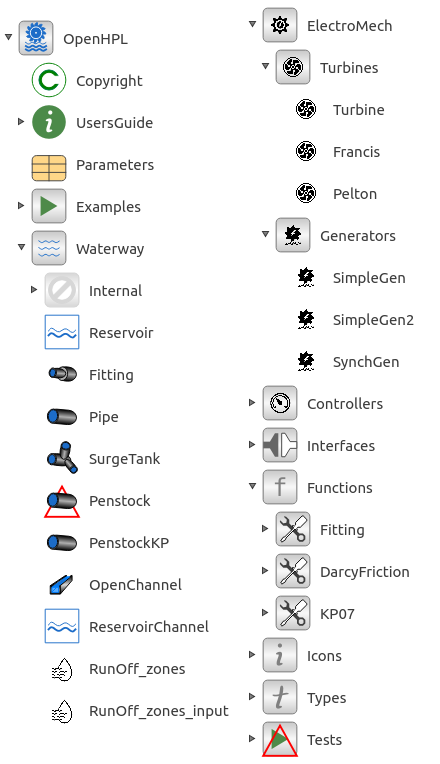
\includegraphics[width=0.7\textwidth]{Library}
 \caption{Screen shot of OpenModelica with the hydropower library.}
  \label{fig:Library}
\end{figure}

The library is divided into various packages:
\begin{description}
\item[\texttt{Copyright}] A documentation class that  provides a reference to the license for this library.
\item[\texttt{UsersGuide}] A documentation class that  provides the user's guide of this library.
\item[\texttt{Data}] A record that determines the common data set for this library. It is possible to insert this class into models and use the common data set for the whole model.
    \item[\texttt{Examples}] A package that provides various examples of using the library for hydropower system as well as examples of using \emph{OpenHPL} together with power system library --- \emph{OpenIPSL}.
    \item[\texttt{Waterway}] A package that consists of various unit models for the waterway of the hydropower system, such as reservoirs, conduits, surge tank, pipe fittings, etc.
    \item[\texttt{ElectroMech}] A package that provides the electro-mechanical components of the hydropower system and consists of two main sub-packages:
      \begin{description}
      \item[\texttt{Turbines}] with various turbine unit models
      \item[\texttt{Generators}] with simplified models of a generator
      \end{description}
    \item[\texttt{Controllers}] A package that holds a simple model for a governor of the hydropower system.
    \item[\texttt{Interfaces}] A package of gives connector interfaces for the library components.
    \item[\texttt{Functions}] A package of functions that consists of three sub-packages:
      \begin{itemize}
      \item[\texttt{Fitting}] Functions for calculation of pressure drop for various pipe fittings.
      \item[\texttt{DarcyFriction}] Functions to calculate the friction term in the pipe.
      \item[\texttt{KP07}] Functions for PDEs using Kurganov-Petrova (KP) scheme.
      \end{itemize}
    \item[\texttt{Icons}] Package of icons used in the library.
    \item[\texttt{Types}] Package of types used in the library.
    \item[\texttt{Tests}] Package of various testing models. Not guaranteed to work and meant for development only.
    \end{description}
Below, a detailed description of each unit model of the \emph{OpenHPL} is provided.

\section{Interfaces}

First, a detailed description of the interface connectors is provided here. In the \emph{OpenHPL}, two types of connectors are typically used.The first type is the standard Modelica real input/output connector, the other type is a set of connectors that represent the water flow and are modelled similar to the connection in an electrical circuit with voltage and current, or similar to the idea of potential and flow in Bond Graph models. The water flow connector which is called \emph{Contact} in the library, contains information about the pressure in the connector and mass flow rate that flows through the connector. An example of a Modelica code for defining the \emph{Contact} connector looks as follows:

\begin{lstlisting}[language = modelica]
connector Contact "Water flow connector"
  Modelica.SIunits.Pressure p "Contact pressure";
  flow Modelica.SIunits.MassFlowRate m_dot "Mass flow rate through the contact";
  // Creating an icon for connector
  annotation (Icon(graphics={  Ellipse(extent={{-100,-100},{100,100}}, lineColor = {28, 108, 200}, fillColor = {0, 128, 255}, fillPattern = FillPattern.Solid)}));
end Contact;
\end{lstlisting}

In addition, some extensions of this water flow connector are developed for the better use in the library. These extensions are listed hereby.
\begin{itemize}
    \item \emph{TwoContact} is an extension from the \emph{Contact} model which provides a model of two connectors of inlet and outlet contacts. A Modelica code for this model looks as follows:
    \begin{lstlisting}[language = modelica]
    partial model TwoContact "Model of two connectors"
      // Specifying connectors and their placement in diagram
      Contact i "Inlet contact" annotation(Placement(transformation(extent={{-110,-10},{-90,10}})));
      Contact o "Outlet contact" annotation(Placement(transformation(extent={{90,-10},{110,10}})));
    end TwoContact;
    \end{lstlisting}
    \item \emph{ContactPort} is an extension from the \emph{TwoContact} model which also provides information about a mass flow rate between these two connectors. The mass flow rate that flows through the inlet connector is equal to the mass flow through the outlet connector. This model is used for the pipe modelling. A Modelica code for this \emph{ContactPort} model looks as follows:
    \begin{lstlisting}[language = modelica]
    partial model ContactPort "Model of two connectors with mass flow rate"
      Modelica.SIunits.MassFlowRate m_dot "Mass flow rate";
      extends TwoContact;
    equation
      0 = i.m_dot + o.m_dot;
      m_dot = i.m_dot;
    end ContactPort;
    \end{lstlisting}
    \item \emph{ContactNode} is an extension from the \emph{TwoContact} model and provides a node pressure that is equal to the pressures from these two connectors. This model also defines the mass flow rate that is the sum of the mass flow rates through the inlet and outlet connectors. This model is used for the surge tank modelling. A Modelica code for this \emph{ContactNode} model looks as follows:
    \begin{lstlisting}[language = modelica]
    partial model ContactNode "Model of two connectors and node pressure"
      Modelica.SIunits.Pressure p_n "Node pressure";
      Modelica.SIunits.MassFlowRate m_dot "Mass flow rate";
      extends TwoContact;
    equation
      p_n = i.p;
      i.p = o.p;
      m_dot = i.m_dot + o.m_dot;
    end ContactNode;
    \end{lstlisting}
    \item \emph{TurbineContacts} is an extension from \emph{ContactPort} model and provides the real input and output connectors, additionally. This model is used for turbine modelling. A Modelica code for this \emph{TurbineContacts} model looks as follows:
    \begin{lstlisting}[language = modelica]
    partial model TurbineContacts "Model of turbine connectors"
      extends ContactPort;
      // Specifying additional connectors and their placement in diagram
      input Modelica.Blocks.Interfaces.RealInput u_t "[Guide vane|nozzle] opening of the turbine" annotation (Placement(transformation(extent = {{-20, -20}, {20, 20}}, rotation = -90, origin={0,120})));
      Modelica.Blocks.Interfaces.RealOutput P_out "Mechanical Output power" annotation (Placement(transformation(origin={0,-110}, extent={{-10,-10},{10,10}}, rotation = 270)));
    end TurbineContacts;
    \end{lstlisting}
\end{itemize}

\section{Functions}

Here, a detailed description of the functions and their used algorithms in the library, are presented.

\subsection{Friction term}

First, the functions for defining the friction force in the waterway are described. More details can be found in Bernt Lie's Lecture notes, \cite{LieL:18}.

The friction force $F_\mathrm{f}$ is directed in the opposite direction of the velocity $v$ (the linear velocity average across the cross-section of the pipe) of the fluid, \cite{LieL:18}. A common expression for friction force in the filled pipes is the following:

\begin{equation}\label{eq:eq1}
    F_\mathrm{f}=-\frac{1}{8}\pi\rho LDf_\mathrm{D}v|v|
\end{equation}
Here, $L$ and $D$ are related to the pipe width and diameter, respectively. $f_\mathrm{D}$ is a Darcy friction factor that is a function of Reynolds number $N_\mathrm{Re}$, with the roughness ratio $\frac{\epsilon}{D}$ as a parameter, see Figure~\ref{fig:fig2}.

In Figure~\ref{fig:fig2}, the turbulent region ($N_\mathrm{Re} > 2.3\cdot10^3$) is a flow regime where the velocity across the pipe has a stochastic nature, and where the velocity $v$ is relatively uniform across the pipe when we average the velocity over some short period of time. The laminar region ($N_\mathrm{Re} < 2.1\cdot10^3$) is a flow regime with a regular velocity v which varies as a parabola with the radius of the pipe, with zero velocity at the pipe wall and maximal velocity at the centre of the pipe.
\begin{figure}[!ht]
  \centering
 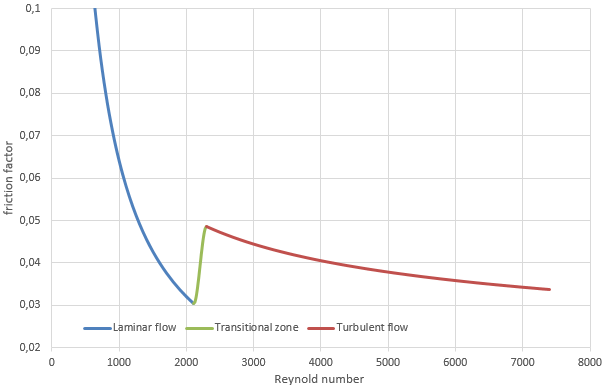
\includegraphics[width=0.8\textwidth]{fig/darcyf}
 \caption{Darcy friction factor as a function of the Reynolds number.}
  \label{fig:fig2}
\end{figure}

Darcy friction factor varies with the roughness of the pipe surface, specified by roughness height $\epsilon$. For laminar flow in a cylindrical pipe ($N_\mathrm{Re} < 2.1\cdot10^3$), the Darcy friction factor $f_\mathrm{D}$ can be found using the following expression:
\begin{equation}\label{eq:eq2}
f_\mathrm{D}=\frac{64}{N_\mathrm{Re}}
\end{equation}
Here, the Reynolds number is found as follows: $N_\mathrm{Re}=\frac{\rho|v|D}{\mu}$, where $\mu$ is the the fluid viscosity.

For turbulent flow ($N_\mathrm{Re} > 2.3\cdot10^3$), it is common to rewrite the expression for the Darcy friction factor as
\begin{equation}\label{eq:eq3}
f_\mathrm{D}=\frac{1}{\left(2\log_{10} \left(\frac{\epsilon}{3.7D} + \frac{5.74}{N_\mathrm{Re}^{0.9}}\right)\right)^ 2}
\end{equation}
In order to define the Darcy friction factor in a region between laminar and turbulent flow regimes, a possibility is to use some interpolation expressions between the laminar value at $N_\mathrm{Re}=2100$ and the turbulent value at $N_\mathrm{Re}= 2300$, e.g., a cubic polynomial fitting with the same slope as laminar friction at $N_\mathrm{Re}=2100$ and turbulent friction at $N_\mathrm{Re}=2300$, \cite{LieL:18}. To achieve the global differentiability, with $p(N_\mathrm{Re})=aN_\mathrm{Re}^3+bN_\mathrm{Re}^2+cN_\mathrm{Re}+d$, thus:
\begin{equation}
\begin{array}{c}
p(N_\mathrm{Re}=2100)=f_\mathrm{D}^\mathrm{l}(N_\mathrm{Re}=2100)\\
p(N_\mathrm{Re}=2300)=f_\mathrm{D}^\mathrm{t}(N_\mathrm{Re}=2300)\\
\left.\frac{dp}{dN_\mathrm{Re}}\right\rvert_{N_\mathrm{Re}=2100}=\left.\frac{df_\mathrm{D}^\mathrm{l}}{dN_\mathrm{Re}}\right\rvert_{N_\mathrm{Re}=2100}\\
\left.\frac{dp}{dN_\mathrm{Re}}\right\rvert_{N_\mathrm{Re}=2300}=\left.\frac{\partial f_\mathrm{D}^\mathrm{t}}{\partial N_\mathrm{Re}}\right\rvert_{\frac{\epsilon}{D},N_\mathrm{Re}=2300}
\end{array}
\end{equation}
Hence, the constants $a$, $b$, $c$ and $d$ can be found as follows:
\begin{equation}\label{eq:eq4}
\begin{bmatrix}a\\b\\c\\d \end{bmatrix}=
\begin{bmatrix}2100^3&2100^2 & 2100& 1\\ 2300^3 & 2300^2 & 2300 & 1\\ 3\cdot2100^2 & 2\cdot2100& 1 & 0\\ 3\cdot2300^2 & 2\cdot2300 &1 & 0\end{bmatrix}^{-1}
\begin{bmatrix} \frac{64}{2100} \\ \frac{1}{\left(2\log_{10}\left(\frac{\epsilon}{3.7D}+\frac{5.74}{2300^ {0.9}}\right)\right)^2} \\ -\frac{64}{2100^ 2} \\ -0.25\frac{0.316}{2300^{1.25}} \end{bmatrix}
\end{equation}
Based on the presented equation for calculation of the friction force in the waterway, two functions are encoded in this class \emph{DarcyFriction}. The first function is for defining the Darcy friction factor and called \emph{fDarcy}. This function has the following inputs: the Reynolds number $N_\mathrm{Re}$, the pipe diameter $D$, and the pipe roughness height $\epsilon$. Then, based on Eq.~\ref{eq:eq2} for the laminar flow (Reynolds number < 2100), Eq.~\ref{eq:eq3} for turbulent flow (Reynolds number > 2300), and Eq.~\ref{eq:eq4} for transitional zone (2100 < Reynolds number < 2300); the \emph{fDarcy} function provides value for the Darcy friction factor $f_\mathrm{D}$.

Another function, \emph{Friction} is for defining the actual friction force and is based on a response from the \emph{fDarcy} function. This function has the following inputs: the linear velocity $v$, the pipe length and diameter $L$ and $D$, the liquid density and viscosity $\rho$ and $\mu$, and the pipe roughness height $\epsilon$. As an output, this function provides a value for the friction force $F_\mathrm{f}$ based on Eq.~\ref{eq:eq1}. An example of a Modelica code for defining the \emph{Friction} function looks as follows:

\begin{lstlisting}[language = modelica]
function Friction "Friction force with Darcy friction factor"
  import Modelica.Constants.pi;
  input Modelica.SIunits.Velocity v "Flow velocity";
  input Modelica.SIunits.Diameter D "Pipe diameter";
  input Modelica.SIunits.Length L "Pipe length";
  input Modelica.SIunits.Density rho "Density";
  input Modelica.SIunits.DynamicViscosity mu "Dynamic viscosity of water";
  input Modelica.SIunits.Height eps "Pipe roughness height";
  // Function output (response) value
  output Modelica.SIunits.Force F_f "Friction force";
// Local (protected) quantities
protected
  Modelica.SIunits.ReynoldsNumber N_Re "Reynolds number";
  Real f "friction factor";
algorithm
  N_Re := rho * abs(v) * D / mu;
  f := fDarcy(N_Re, D, eps);
  F_f := 0.5 * pi * f * rho * L * v * abs(v) * D / 4;
end Friction;
\end{lstlisting}

\subsection{KP scheme}

Here, functions for solving PDEs in Modelica are described. First, the overview of the KP scheme is presented. More details about this scheme can be found in Roshan Sharma work, \cite{Sha:15}, and other works, \cite{Vyt:15,Vyt:17}.

This is a well-balanced second-order scheme, which is a Reimann problem solver free scheme (central scheme) while at the same time, it takes advantage of the upwind scheme by utilizing the local, one side speed of propagation (given by the eigenvalues of the Jacobian matrix) during the calculation of the flux at the cell interfaces, \cite{Sha:15}.

The central-upwind numerical scheme is presented for the one-dimensional case.
\begin{equation}
\frac{\partial U\left(x,t\right)}{\partial t}+\frac{\partial F\left(x,t,U\right)}{\partial x}=S\left(x,t,U\right)
\end{equation}
Here, $U\left(x,t\right)$ is the state vector, where states are the functions of position $x$ and time $t$. $F\left(x,t,U\right)$ is the vector of fluxes and $S\left(x,t,U\right)$ is the source terms.

In order to solve this PDE, it should be first discretized by finite-volume methods. With the finite volume method, we divide the grid into small control volumes/cells and then apply the conservation laws. This control volume/cell with notations are shown in Figure~\ref{fig:fig2_1}.
\begin{figure}[!ht]
  \centering
 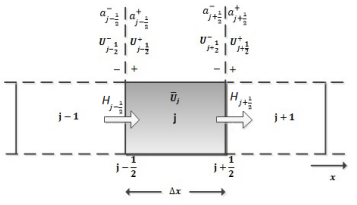
\includegraphics[width=0.7\textwidth]{fig/kp}
 \caption{Control volume/cell, \cite{Sha:15}.}
  \label{fig:fig2_1}
\end{figure}

Hence, the semi-discrete (time-dependent ODEs) central-upwind scheme can be then written in the following form:
\begin{equation}\label{eq:eq7}
\frac{d}{dt}\bar{U}_j\left(t\right)=-\frac{H_{j+\frac{1}{2}}\left(t\right)-H_{j-\frac{1}{2}}\left(t\right)}{\Delta x}+\bar{S}_j\left(t\right)
\end{equation}
Here, $\bar{U}_j$ are the cell centre average values, while $H_{j\pm\frac{1}{2}}\left(t\right)$ are the central upwind numerical fluxes at the cell interfaces and are given by:
\begin{equation}\label{eq:eq8}
\begin{array}{c}
H_{j+\frac{1}{2}}\left(t\right)=\frac{a^+_{j+\frac{1}{2}}F\left(U^-_{j+\frac{1}{2}}\right)-a^-_{j+\frac{1}{2}}F\left(U^+_{j+\frac{1}{2}}\right)}{a^+_{j+\frac{1}{2}}-a^-_{j+\frac{1}{2}}}+\frac{a^+_{j+\frac{1}{2}}a^-_{j+\frac{1}{2}}}{a^+_{j+\frac{1}{2}}-a^-_{j+\frac{1}{2}}}\left[U^+_{j+\frac{1}{2}}-U^-_{j+\frac{1}{2}}\right]\\
H_{j-\frac{1}{2}}\left(t\right)=\frac{a^+_{j-\frac{1}{2}}F\left(U^-_{j-\frac{1}{2}}\right)-a^-_{j-\frac{1}{2}}F\left(U^+_{j-\frac{1}{2}}\right)}{a^+_{j-\frac{1}{2}}-a^-_{j-\frac{1}{2}}}+\frac{a^+_{j-\frac{1}{2}}a^-_{j-\frac{1}{2}}}{a^+_{j-\frac{1}{2}}-a^-_{j-\frac{1}{2}}}\left[U^+_{j-\frac{1}{2}}-U^-_{j-\frac{1}{2}}\right]
\end{array}
\end{equation}
Here, $a^\pm_{j\pm\frac{1}{2}}$ are the one-sided local speeds of propagation.

For calculating the numerical fluxes $H_{j\pm\frac{1}{2}}\left(t\right)$, the values of states at the cell interfaces $U^\pm_{j\pm\frac{1}{2}}$ are needed. These values can be calculated as the endpoints of a piecewise linearly reconstructed function:
\begin{equation}\label{eq:eq9}
\begin{array}{c}
U^-_{j+\frac{1}{2}}=\bar{U}_j+\frac{\Delta x}{2}s_j\\
U^+_{j+\frac{1}{2}}=\bar{U}_{j+1}-\frac{\Delta x}{2}s_{j+1}\\
U^-_{j-\frac{1}{2}}=\bar{U}_{j-1}+\frac{\Delta x}{2}s_{j-1}\\
U^+_{j-\frac{1}{2}}=\bar{U}_j-\frac{\Delta x}{2}s_j
\end{array}
\end{equation}
The slope $s_j$ of the reconstructed function in each cell is computed using a limiter function to obtain a non-oscillatory nature of the reconstruction. The KP scheme utilizes the generalized \emph{minmod} limiter as:
\begin{equation}\label{eq:eq10}
\begin{array}{c}
s_j^-=\theta\frac{\bar{U}_j-\bar{U}_{j-1}}{\Delta x},s_j^c=\frac{\bar{U}_{j+1}-\bar{U}_{j-1}}{2\Delta x},s_j^+=\theta\frac{\bar{U}_{j+1}-\bar{U}_{j}}{\Delta x}\\
s_j=minmod\left(s_j^-,s_j^c,s_j^+\right)=\begin{cases}
   \min\left(s_j^-,s_j^c,s_j^+\right), & \text{if }s_j^->0\text{ \& }s_j^c>0\text{ \& }s_j^+>0 \\
   \max\left(s_j^-,s_j^c,s_j^+\right), & \text{if }s_j^-<0\text{ \& }s_j^c<0\text{ \& }s_j^+<0 \\
   0, & \text{otherwise}
  \end{cases}
\end{array}
\end{equation}
The parameter $\theta\in[1,2]$ is used to control or tune the amount of numerical dissipation or numerical viscosity present in the resulting scheme. The value of $\theta = 1.3$ is an acceptable starting point in general.

It can be observed that for a given $j^\mathrm{th}$ cell, the information from the neighbouring cells $j-1$ and $j-2$ (to the left) and $j+1$ and $j+2$ (to the right) are required for calculating the flux integrals. This will pose difficulties at the cells on the left and right boundaries. While evaluating the flux integrals near the left boundary cells ($j=1$ and $j=2$) and near the right boundary cells ($j=N-1$ and $j=N$; $N$ is the number of cells in the grid), imaginary cells that lie outside the physical boundary should also be taken into consideration, see Figure~\ref{fig:fig2_2}.
\begin{figure}[!ht]
  \centering
 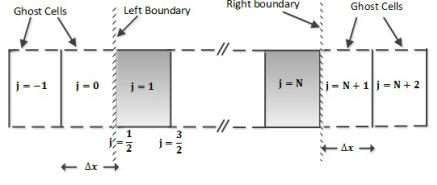
\includegraphics[width=0.7\textwidth]{fig/ghosts}
 \caption{Ghost cells at the grid boundaries, \cite{Sha:15}.}
  \label{fig:fig2_2}
\end{figure}

These imaginary cells denoted by $j=0$ and $j=-1$ on the left, and $j=N+1$ and $j=N+2$ on the right are called the ghost cells. The average value of the conserved variables at the centre of these ghost cells depends on the nature of the physical boundary taken into account. These ghosts cells can be defined in the following way:
\begin{equation}\label{eq:eq11}
\begin{array}{c}
\bar{U}_{j=0}=2\bar{U}_{j=1}-\bar{U}_{j=2}\\
\bar{U}_{j=-1}=2\bar{U}_{j=0}-\bar{U}_{j=1}\\
\bar{U}_{j=N+1}=2\bar{U}_{j=N}-\bar{U}_{j=N-1}\\
\bar{U}_{j=N+2}=2\bar{U}_{j=N+1}-\bar{U}_{j=N}
\end{array}
\end{equation}
The one-sided local speeds of propagation can be estimated as the largest and the smallest eigenvalues $\lambda_{1,2}$ of the Jacobian $\frac{\partial F}{\partial U}$ of the system as:
\begin{equation}\label{eq:eq12}
\begin{array}{c}
a^+_{j\pm\frac{1}{2}}=\max\left(\lambda^+_{1,j\pm\frac{1}{2}},\lambda^-_{1,j\pm\frac{1}{2}},0\right)\\
a^-_{j\pm\frac{1}{2}}=\max\left(\lambda^+_{2,j\pm\frac{1}{2}},\lambda^-_{2,j\pm\frac{1}{2}},0\right)
\end{array}
\end{equation}
Lastly, the source term $\bar{S}_j\left(t\right)$ has to be appropriately discretized to ensure the well-balanced method. This can be written as:
\begin{equation}
\bar{S}_j\left(t\right)=S\left(\bar{U}_j\right)
\end{equation}
Hence, the separate functions for each of these elements defining in Eqs.~\ref{eq:eq8}-\ref{eq:eq12} are modelled and encoded in \emph{OpenHPL}. These functions are assembled in the \emph{KPfunctions} folder in class \emph{KP07}, and look as follows:
\begin{itemize}
\item \emph{GhostsCell} function provides values of the conserved variables at the centre of the ghost cells, using Eq.~\ref{eq:eq11}. As an input piece of information this function receives the number of cells $N$, and the state vector with the cell centre average values $\bar{U}_{j=1..N}$. Then, the \emph{GhostsCell} function returns a state vector with the cell centre average values for all (including ghost) cells $\bar{U}_{j=-1..N+2}$.
\item \emph{SlopeVectoreS} function returns the slope vector $s_{j=0..N+1}$ of the reconstructed function for each cell, using Eq.~\ref{eq:eq10}. This function has the following inputs: the number of cells $N$, parameters $\theta$ and $\Delta x$, and the state vector with the cell centre average values $\bar{U}_{j=-1..N+2}$.
\item Then, function \emph{WiseU} is created to define the values of states $U^\pm_{j\pm\frac{1}{2}}$ as the endpoints of a piecewise linearly reconstructed function from Eq.~\ref{eq:eq9} using the two previous functions. This function has the following inputs: the number of cells $N$, parameters $\theta$ and $\Delta x$, condition and values for the boundaries, and the state vector with the cell centre average values $\bar{U}_{j=1..N}$.
\item Another function as the \emph{SpeedPropagationApipe} provides the one-sided local speeds of propagation $a^\pm_{j\pm\frac{1}{2}}$, using Eq.~\ref{eq:eq12}. As an input information this function receives the number of cells $N$ and vectors of eigenvalues $\lambda^\pm_{1,j\pm\frac{1}{2}}$ and $\lambda^\pm_{2,j\pm\frac{1}{2}}$ of the Jacobian of the system.
\item The last function \emph{FluxesH} in the \emph{KPfunctions} folder, defines the central upwind numerical fluxes at the cell interfaces  $H_{j\pm\frac{1}{2}}$, using Eq.~\ref{eq:eq8}. This function has the following inputs: the number of cells $N$, the values of states at the cell interfaces $U^\pm_{j\pm\frac{1}{2}}$, the one-sided local speeds of propagation $a^\pm_{j\pm\frac{1}{2}}$, and the vector of fluxes $F\left(U^\pm_{j\pm\frac{1}{2}}\right)$.
\end{itemize}

Then, the primary function for the KP scheme \emph{KPmethod} is created which uses the last three presented functions to define the right-hand side of Eq.~\ref{eq:eq7} (discretization solution of PDE).  As an input piece of information, this function receives the number of cells $N$, parameters $\theta$ and $\Delta x$, the state vector with the cell centre average values $\bar{U}_{j=1..N}$, vectors of eigenvalues $\lambda^\pm_{1,j\pm\frac{1}{2}}$ and $\lambda^\pm_{2,j\pm\frac{1}{2}}$ of the Jacobian of the system, the vector of fluxes $F\left(U^\pm_{j\pm\frac{1}{2}}\right)$ and source terms $\bar{S}_j$, and condition and values for the boundaries. It should be noted that the \emph{KPmethod} function is encoded for the cases of systems with two states (state vector $\bar{U}_{j=1..N}$ consists of two states) that is common for the detailed model of the pipe or open channel model (see those unit models below). The boundaries are specified with the inlet and outlet state values: either inlet (or: outlet) values for both states, or inlet and outlet values for one of the states.

In the case with the use of the KP scheme for the open channel model \cite{Sha:15,Vyt:15}, one of the states should be processed through the scheme with some additional vector that is ensured in this \emph{KPmethod} function ($B_{j=-1..N+2}$ vector is also input to the functions \emph{KPmethod} and \emph{WiseU}).

It should be noted that due to the issues of the simulation speed, all of the presented functions in class \emph{KP07} are implemented as the \emph{model} type in OpenModelica instead of the \emph{function} type. An example of a Modelica code for defining the \emph{KPmethod} function looks as follows:

\begin{lstlisting}[language = modelica]
model KPmethod
  extends Icons.Method;
  parameter Integer N "number of segments";
  input Real U[2 * N] "state vector",
             dx "length step",
             theta = 1.3 "parameter for slope limiter",
             S_[2 * N] "source term vector S",
             F_[2 * N, 4] "vector F",
             lam1[N, 4] "matrix of eigenvalues '+'",
             lam2[N, 4] "matrix of eigenvalues '-'",
             B[N + 4] = zeros(N + 4) "additional for open channel",
             boundary[2, 2] "values for boundary conditions";
  input Boolean boundaryCon[2, 2] "boundary conditions consideration";
  output Real diff_eq[2 * N] "right hand side for KP solution";
  Real U_[8, N] "matrix with boundary state values. Can be extracted";
protected
  Real H_[2 * N, 2] "matrix of fluxes",
       A_speed[N, 4] "matrix of one-side local speeds propagation";
public
  KPfunctions.WiseU wiseU(N = N, theta = theta, U = U, B = B, dx = dx, boun = boundary, bounCon = boundaryCon) "use function for defing the piece wise linear reconstruction of vector U";
  KPfunctions.SpeedPropagationApipe speedA(N = N, lamda1 = lam1, lamda2 = lam2) "use function for defing the one-side local speeds propagation";
  KPfunctions.FluxesH fluxesH(N = N, U_ = U_, A_ = A_speed, F_ = F_) "use function for defing the central upwind numerical fluxes";
equation
  ///// piece wise linear reconstruction of vector U
  U_ = wiseU.U_;
  ///// one-side local speeds propagation
  A_speed = speedA.A;
  ///// central upwind numerical fluxes
  H_ = fluxesH.H;
  //// right hand side of diff. equation
  diff_eq = (-(H_[:, 1] - H_[:, 2]) / dx) + S_;
end KPmethod;
\end{lstlisting}

Examples of using the KP scheme for solving PDEs are also provided in the class \emph{KP07} in the \emph{TestKPpde} folder. More information about using the \emph{KPmethod} function is presented below in the waterway modelling section for the \emph{PenstockKP} and \emph{OpenChannel} units.

\subsection{Fitting}

The functions for defining the pressure drop in various pipe fittings are described here. More details can be found in Bernt Lie's Lecture notes, \cite{LieL:18}.

Due to different constrictions in the pipes, it is of interest to define losses in these fittings. This can be done based on friction pressure drop which can be calculated as:
\begin{equation}\label{eq:eq14}
\Delta p_\mathrm{f}=\frac{1}{2}\phi\rho v|v|
\end{equation}
Here, the dimensionless factor $\phi$ is $\phi=f_\mathrm{D}\frac{L}{D}$ for a long, straight pipe. Here, $\phi$ will be the generalized friction factor. In this case, it is possible to write pressure drop for different constrictions. Some cases of various fittings are shown in Figures~\ref{fig:fig3}-\ref{fig:fig6}. Equations for the dimensionless factor $\phi$  are also demonstrated in these figures for the presented fittings.
\begin{figure}[!ht]
  \centering
 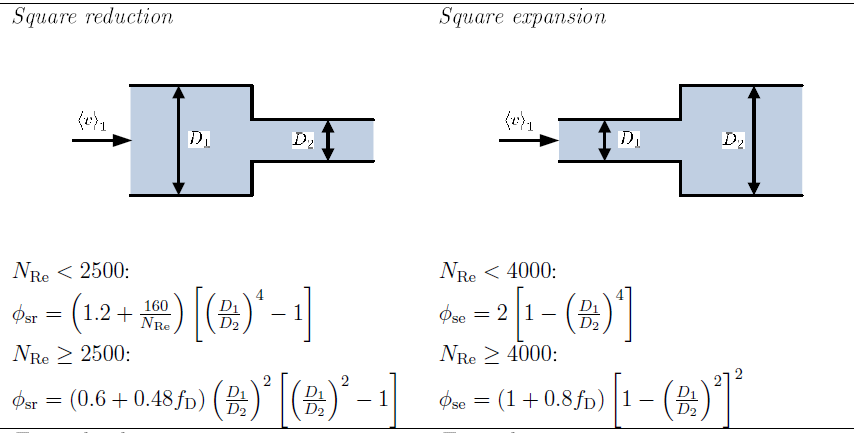
\includegraphics[width=0.8\textwidth]{fig/Square_fi}
 \caption{Square reduction/expansion fittings, \cite{LieL:18}.}
  \label{fig:fig3}
\end{figure}
\begin{figure}[!ht]
  \centering
 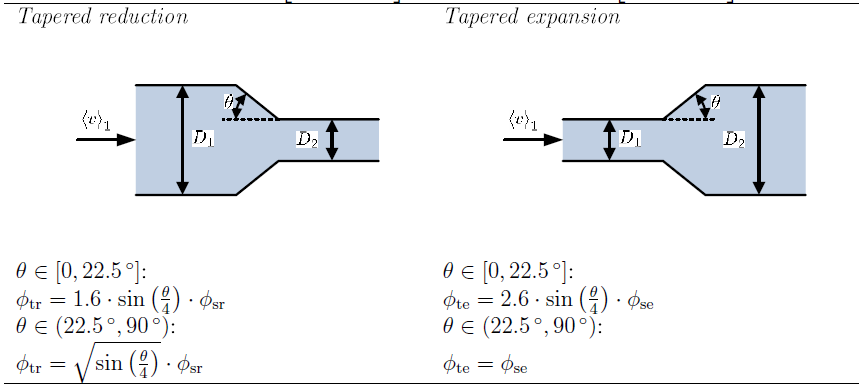
\includegraphics[width=0.8\textwidth]{fig/Tapered_fit}
 \caption{Tapered reduction/expansion fittings, \cite{LieL:18}.}
  \label{fig:fig4}
\end{figure}
\begin{figure}[!ht]
  \centering
 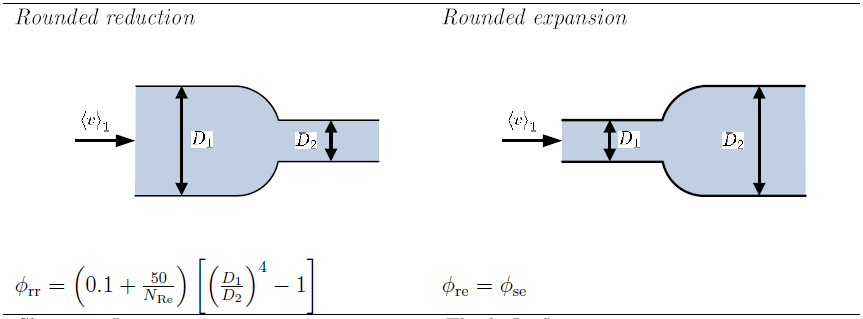
\includegraphics[width=0.8\textwidth]{fig/Rounded_fit}
 \caption{Rounded reduction/expansion fittings, \cite{LieL:18}.}
  \label{fig:fig5}
\end{figure}
\begin{figure}[!ht]
  \centering
 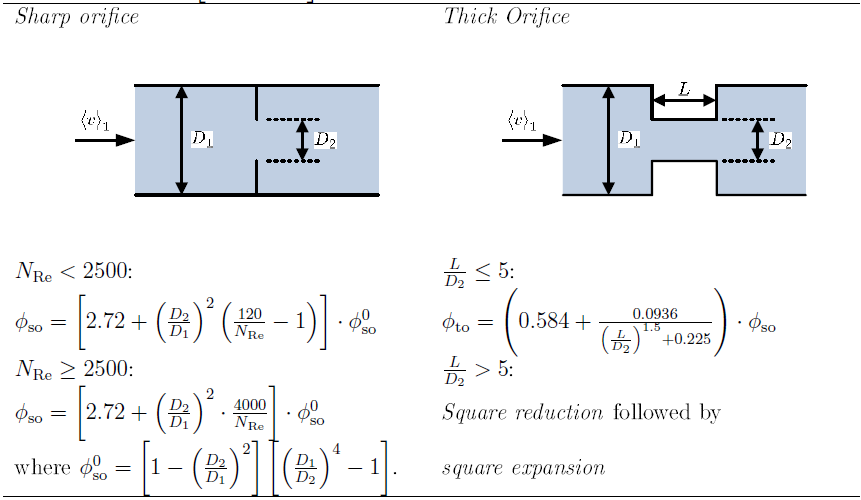
\includegraphics[width=0.8\textwidth]{fig/Sharp_fit}
 \caption{Sharp/Thick orifice fittings, \cite{LieL:18}.}
  \label{fig:fig6}
\end{figure}

Based on the presented equations and figures for the calculation of the dimensionless factor $\phi$ in the various fitting, a set of functions is encoded regarding each specific type of fittings, such as \emph{SquareReduction}, \emph{SquareExpansion}, \emph{TaperedReduction}, \emph{TaperedExpansion}, \emph{RoundedReduction}, \emph{SharpOrifice}, and \emph{ThickOrifice}. All these functions receive the Reynolds number $N_\mathrm{Re}$, diameters of first and second pipes $D_1$ and $D_2$, and the pipe roughness height $\epsilon$. Then, based on the equations from Figures~\ref{fig:fig3}-\ref{fig:fig6}, these functions provide value for the dimensionless factor $\phi$. As an example, a Modelica code for defining the \emph{SquareReduction} function looks as follows:

\begin{lstlisting}[language = modelica]
function SquareReduction
  input Modelica.SIunits.ReynoldsNumber N_Re "Reynolds number";
  input Modelica.SIunits.Height eps "Pipe roughness height";
  input Modelica.SIunits.Diameter D_i, D_o "Pipe diameters";
  output Real phi;
protected
  Real f_D "friction factor";
algorithm
  f_D := Functions.DarcyFriction.fDarcy(N_Re, D_1, eps);
  if N_Re < 2500 then
    phi := (1.2 + 160 / N_Re) * ((D_i / D_o) ^ 4 - 1);
  else
    phi := (0.6 + 0.48 * f_D) * (D_i / D_o) ^ 2 * ((D_i / D_o) ^ 2 - 1);
  end if;
end SquareReduction;
\end{lstlisting}

Another function, \emph{FittingPhi} also provides the dimensionless factor $\phi$ as an output. This function calls the presented above functions with a specific type of the fitting in order to get value for the factor $\phi$. This function has the following inputs: the linear velocity $v$, the pipe length $L$, diameters of first and second pipes $D_i$ and $D_o$, liquid density and viscosity $\rho$ and $\mu$, the pipe roughness height $\epsilon$. The last input for this function is a variable with the specific type \emph{FittingType} that holds information about the fitting type.

\section{Waterway}

A typical structure of the waterway of the hydropower system is shown in Figure~\ref{fig:fig7}.

\begin{figure}[!ht]
  \centering
 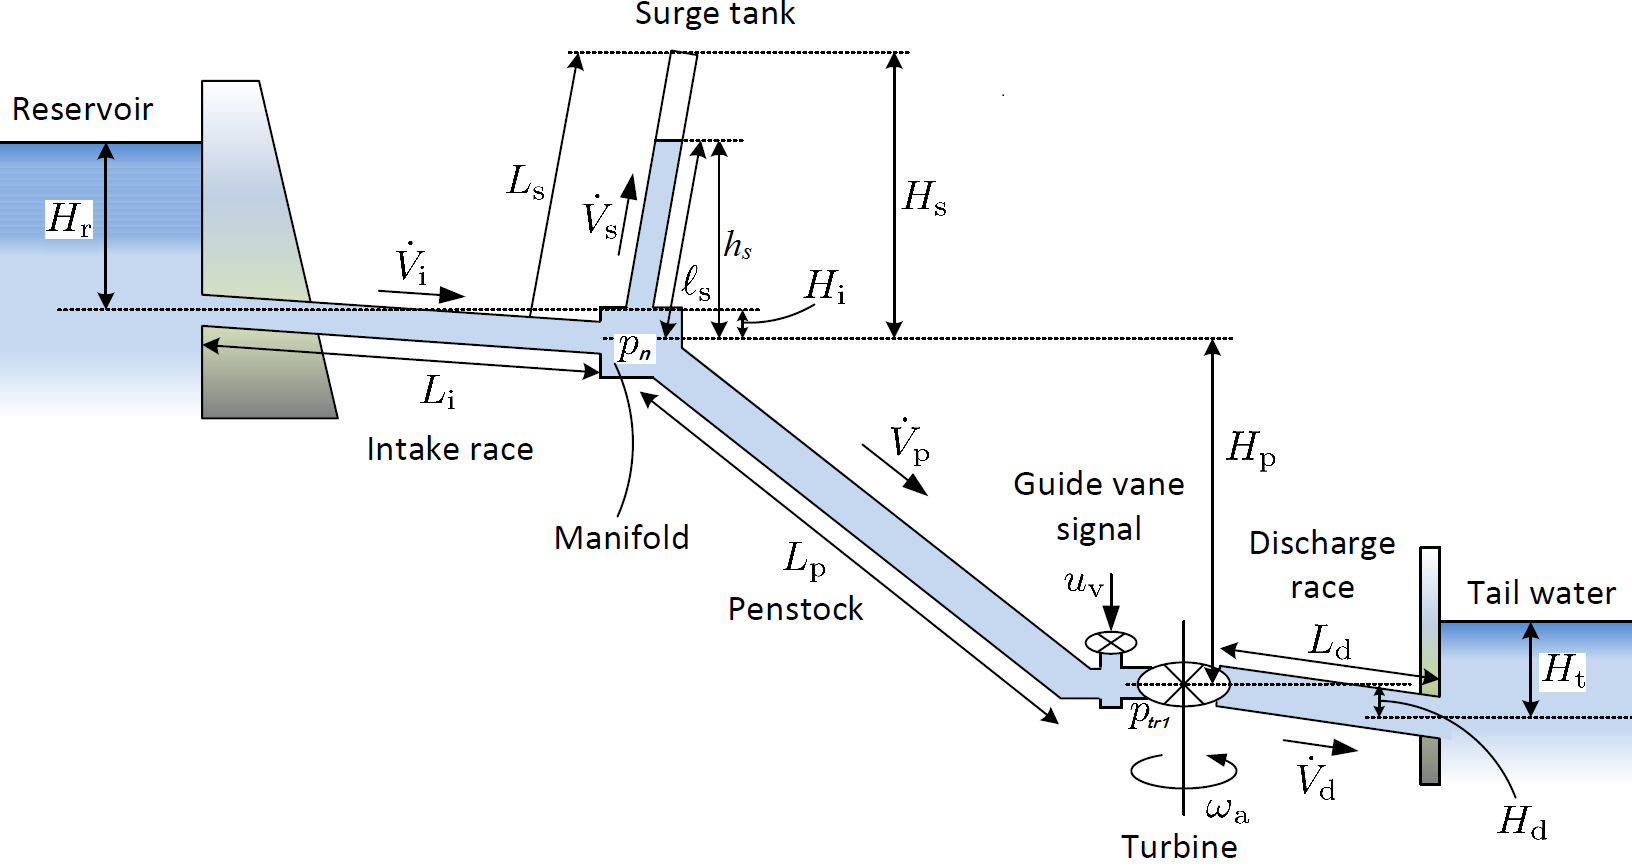
\includegraphics[width=0.95\textwidth]{fig/Fig_1_scheme}
 \caption{Reservoir structure, \cite{LieL:18}.}
  \label{fig:fig7}
\end{figure}

\subsection{Reservoir}

Figure~\ref{fig:fig7} shows that the water level in the reservoir $H_\mathrm{r}$ is a key quantity, \cite{Val:17}. Similarly to the water tank, a reservoir model can be described by mass and momentum balances as following, \cite{Sha:11}:
\begin{equation}
\begin{array}{c}
    H_\mathrm{r}\frac{d\dot{m}_\mathrm{r}}{dt}=\frac{\rho}{A_\mathrm{r}}\dot{V}_\mathrm{r}^2+A_\mathrm{r}\left(p_\mathrm{atm}-p_\mathrm{r}\right)+\rho gH_\mathrm{r}A_\mathrm{r}-F_\mathrm{f,r}\\
    \frac{dm_\mathrm{r}}{dt}=\dot{m}_\mathrm{r}
\end{array}
\end{equation}
Here, $\dot{m}_\mathrm{r}$ is the reservoir mass flow rate that can be found from the reservoir volumetric flow rate $\dot{V}_\mathrm{r}$. $A_\mathrm{r}$ is a square area of the reservoir. $p_\mathrm{atm}$ and $p_\mathrm{r}$ are the atmospheric and the reservoir outlet pressures, respectively. $F_\mathrm{f,r}$ is a friction term that can be found using Darcy friction factor.

In a simple case, it can be assumed that the level of the reservoir is constant, the reservoir inlet flow equal the outlet flow, and the area of the reservoir is closed to infinity. Then the reservoir can be presented just as an equation for pressure in the inlet/outlet of the reservoir, \cite{Sha:11,Val:17}.
\begin{equation}
    p_\mathrm{r}=p_\mathrm{atm}+\rho gH_\mathrm{r}
\end{equation}
Hence, both of these cases are modelled in the \emph{Reservoir} unit in the library. This unit uses the \emph{Contact} connector and can be connected to other waterway units. The \emph{Reservoir} unit can be specified with the following options:
\begin{itemize}
    \item The user can choose a simple model of the reservoir, and calculate the outlet pressure depending on the depth of the outlet from the reservoir.
    \item The user can also choose a more complicated model, add the inflow to the reservoir and specify the reservoir geometry.
    \item Also, it is possible to connect an input signal with the varying water level in the reservoir.
\end{itemize}

\subsection{Fitting}

There are various possibilities of the fittings for the pipes with different diameters as well as the existence of orifices in the pipe. In this unit \emph{Fitting}, the pressure drop due to these constrictions is defined using Eq.~\ref{eq:eq14} and function \emph{FittingPhi}. The \emph{Fitting} unit uses the \emph{ContactPort} connector model in order to have inlet and outlet connectors and the possibility to define pressure drop between those connectors. Then, this unit can be connected to the other waterway units.

When the \emph{Fitting} unit is in use, the user can postulate the specific type of fitting that is of interest and required based on the geometry parameters for this fitting.

\subsection{Pipe}

The simple model of the pipe unit \emph{Pipe} gives possibilities for easy modelling of different conduit: intake race, penstock, tailrace, etc. In these waterway units, there are only small pressure variations due to the small slope angle (height difference between inlet and outlet of the component). That is why the model for these units can be simplified by considering incompressibility of the water and the inelasticity of the walls, \cite{Vyt:17,Val:17,Sha:11}. A sketch of the pipe with all needed terms for modelling is shown in Figure~\ref{fig:fig8}.
\begin{figure}[!ht]
  \centering
 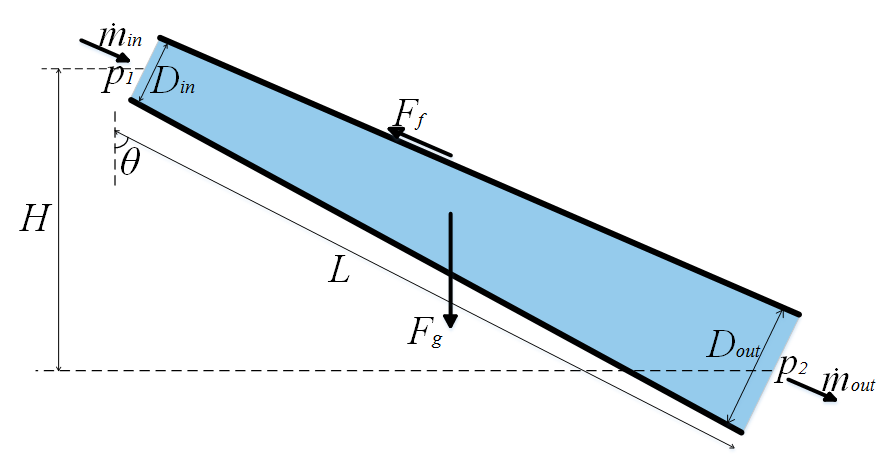
\includegraphics[width=0.6\textwidth]{fig/Fig_2_scheme}
 \caption{Model for flow through a pipe.}
  \label{fig:fig8}
\end{figure}

In the case of incompressible water, the mass in the filled pipe is constant, and:
\begin{equation}\label{eq:eq17}
\frac{dm_\mathrm{c}}{dt} = \dot{m}_\mathrm{c,in} - \dot{m}_\mathrm{c,out} = 0
\end{equation}
Here, the mass of the water in the pipe (conduit) is $m_\mathrm{c}=\rho V_\mathrm{c}=\rho L_\mathrm{c}\overline{A}_\mathrm{c}$, where $\rho$ is the water density, $V_c$ -- the volume of the water in the pipe, $L_\mathrm{c}$ -- the length of the pipe (conduit) and $\overline{A}_\mathrm{c}$ -- the averaged cross-section area of the pipe that are defined from averaged pipe diameter $\overline{D}_\mathrm{c}$. The inlet and outlet mass flow rates are equal with $\dot{m}_\mathrm{c,in}=\rho\dot{V}_\mathrm{c,in}$ and $\dot{m}_\mathrm{c,out}=\rho\dot{V}_\mathrm{c,out}$ respectively, where $\dot{V}_\mathrm{c,in}=\dot{V}_\mathrm{c,out}$ -- the inlet and outlet volumetric flow rates in the pipe.

The momentum balance for this simplified model can be expressed as:
\begin{equation}\label{eq:eq18}
\frac{dM_\mathrm{c}}{dt} = \dot{M}_\mathrm{c,in} - \dot{M}_\mathrm{c,out} + F_\mathrm{p,c} + F_\mathrm{g,c} + F_\mathrm{f,c}
\end{equation}
Here, the momentum of the water in the pipe is $M_\mathrm{c}=m_\mathrm{c}v_\mathrm{c}$, where $v_\mathrm{c}$ is the average water velocity and can be defined as $v_\mathrm{c}=\dot{V}_\mathrm{c}/\overline{A}_\mathrm{c}$. The inlet and outlet momentum flow rates are $\dot{M}_\mathrm{c,in}=\dot{m}_\mathrm{c,in}v_\mathrm{c,in}$ and $\dot{M}_\mathrm{c,out}=\dot{m}_\mathrm{c,out}v_\mathrm{c,out}$ respectively, where $v_\mathrm{c,in}=\dot{V}_\mathrm{c,in}/A_\mathrm{c,in}$ and $v_\mathrm{c,out}=\dot{V}_\mathrm{c,out}/A_\mathrm{c,out}$ are the velocities in the inlet and outlet of the pipe, respectively; and are equal in a case with constant diameter of the pipe ($A_\mathrm{c,in}=A_\mathrm{c,out}$). $F_\mathrm{p,c}$ -- the pressure force, due to the difference between the inlet and outlet pressures $p_\mathrm{c,1}$ and $p_\mathrm{c,2}$ can be calculated as follows: $F_\mathrm{p,c}=A_\mathrm{c,in}p_\mathrm{c,1}-A_\mathrm{c,out}p_\mathrm{c,2}$. There is also gravity force that is defined as $F_\mathrm{g,c}=m_\mathrm{c}g\cos\theta_\mathrm{c}$, where $g$ -- the gravitational acceleration and $\theta_\mathrm{c}$ -- the angle of the pipe slope that can be defined from the ratio of height difference $H_\mathrm{c}$ and the length $L_\mathrm{c}$ of the pipe. The last term in the momentum balance is friction force which can be calculated as $F_\mathrm{f,c}=-\frac{1}{8}L_\mathrm{c}f_\mathrm{D,c}\pi\rho\overline{D}_\mathrm{c}v_\mathrm{c}|v_\mathrm{c}|$ using the Darcy friction factor $f_\mathrm{D,c}$ for the conduit.

The main defined variable is the volumetric flow rate. In this \emph{Pipe} unit, the flow rate changes simultaneously in the whole pipe (information about the speed of wave propagation is not included here). Water pressures can be shown just in the boundaries of pipe (inlet and outlet pressure from connectors). This unit uses the \emph{ContactPort} connector model and can be connected to other waterway units.

When the \emph{Pipe} unit is in use, the user can specify the required geometry parameters for this pipe: length $L_\mathrm{c}$, height difference $H_\mathrm{c}$, inlet and outlet diameters $D_\mathrm{c,i}$ and $D_\mathrm{c,o}$, and pipe roughness height $\epsilon_\mathrm{c}$. In order to define the friction force $F_\mathrm{f,c}$ the \emph{Friction} function is used here. It should be noted that this unit provides possibilities for the modelling of pipes with both positive and negative slopes (positive or negative height difference). This unit can be initialized by the initial value of the flow rate $\dot{V}_\mathrm{c,0}$. Otherwise, user can choose to an option when the simulation starts from steady-state and the OpenModelica handles automatically initial steady-state values (does not work properly in OpenModelica).

\subsection{Surge Tank}

The surge shaft/tank will be presented here as a vertical open pipe with constant diameter together with manifold, which connecting conduit, surge volume and penstock, \cite{Sha:11,Val:17}. Surge volume (vertical open pipe) is shown in Figure~\ref{fig:fig9}.
\begin{figure}[!ht]
  \centering
 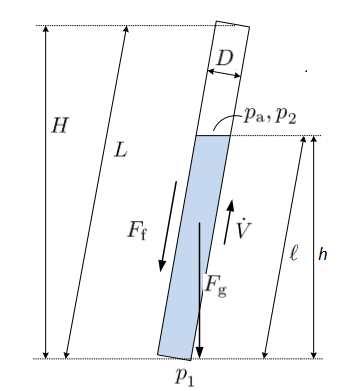
\includegraphics[width=0.4\textwidth]{fig/surgepic}
 \caption{Model for a vertical open pipe.}
  \label{fig:fig9}
\end{figure}

The model for the surge volume can be described by mass and momentum balances as follows:
\begin{equation}
\begin{array}{c}
\frac{dm_\mathrm{s}}{dt} = \dot{m}_\mathrm{s,in} = \rho \dot{V}_\mathrm{s}\\
\frac{dm_\mathrm{s}v_\mathrm{s}}{dt} =\dot{m}_\mathrm{s,in}v_\mathrm{s,in}+F_\mathrm{p,s}+F_\mathrm{g,s}+F_\mathrm{f,s}
\end{array}
\end{equation}
Here, the mass of the water in the surge tank is $m_\mathrm{s}=\rho V_\mathrm{s}=\rho l_\mathrm{s}A_\mathrm{s}=\rho A_\mathrm{s}\frac{h_\mathrm{s}}{\cos\theta_\mathrm{s}}$, where $\rho$ is the water density, $V_s$ is the volume of the water in the surge tank, $h_\mathrm{s}$ and $l_\mathrm{s}$ are the height and length of the surge tank filled with water and $A_\mathrm{s}$ is the cross-section area of the surge tank that defined from the vertical pipe diameter $D_\mathrm{s}$.  The water velocity $v_\mathrm{s}$ can be defined as $v_\mathrm{s}=\dot{V}_\mathrm{s}/A_\mathrm{s}$. The inlet water velocity $v_\mathrm{s,in}=\dot{V}_\mathrm{s}/A_\mathrm{s}$. $F_\mathrm{p,s}$ is the pressure force, due to the difference between the inlet and outlet pressures $p_\mathrm{s,1}$ and $p_\mathrm{atm}$ and can be calculated as follows: $F_\mathrm{p,s}=A_\mathrm{s}\left(p_\mathrm{s,1}-p_\mathrm{atm}\right)$. There is also gravity force that is defined as $F_\mathrm{g,s}=m_\mathrm{s}g\cos\theta_\mathrm{s}$, where $g$ -- the gravitational acceleration and $\theta_\mathrm{s}$ -- the angle of the slope of the surge tank and can be defined from the ratio of height difference $H_\mathrm{s}$ and length $L_\mathrm{s}$. The last term in the momentum balance is friction force, which can be calculated as $F_\mathrm{f,s}=-\frac{1}{8}l_\mathrm{s}f_\mathrm{D,s}\pi\rho D_\mathrm{s}v_\mathrm{s}|v_\mathrm{s}|$ using Darcy friction factor $f_\mathrm{D,s}$ for the surge tank.

The manifold is described by the preservation of mass in steady-state; the volumetric flow rate in the intake race $\dot{V}_\mathrm{i}$ equals to the sum of volumetric flow rates from surge volume $\dot{V}_\mathrm{s}$ and penstock $\dot{V}_\mathrm{p}$: $\dot{V}_\mathrm{i}=\dot{V}_\mathrm{p}+\dot{V}_\mathrm{s}$. In addition, the manifold pressure is equal for all three connections. This manifold is already implemented in the \emph{ContactNode} connectors model that is used in this \emph{SurgeTank} unit. Then, this unit can be connected to other waterway units.

In the \emph{SurgeTank} unit, the user can specify the required geometry parameters for the surge tank (vertical pipe): length $L_\mathrm{s}$, height difference $H_\mathrm{s}$, diameters $D_\mathrm{s}$, pipe roughness height $\epsilon_\mathrm{s}$, and value for the atmospheric pressure $p_\mathrm{atm}$. In order to define the friction force $F_\mathrm{f,s}$ the \emph{Friction} function is used here. This unit can be initialized by the initial values of the flow rate $\dot{V}_\mathrm{s,0}$ and water height $h_\mathrm{s,0}$. Otherwise, the user can decide on an option when the simulation starts from the steady-state and the OpenModelica automatically handles the initial steady-state values (does not work properly in OpenModelica).

\subsection{Pipe with compressible water and elastic walls}

Unlike the conduit, the penstock has considerable pressure variation due to a considerable height drop. Thus, to make the model for the penstock more realistic, the compressible water and the elastic walls of the penstock should be taken into account. To express the compressibility/elasticity, some compressibility coefficients which show the relationship between pressure, water density and pipe inner radius, are used, \cite{Sha:11,Vyt:17}.

The isothermal compressibility $\beta_T$ is defined as follows:
\begin{equation}
\beta_T = \frac{1}{\rho}\frac{d\rho}{dp}
\end{equation}
Here, $\rho$ and $p$ denote density and pressure, respectively. Assuming that the isothermal compressibility is independent of the pressure, this equation can be rewritten in a way that is convenient to calculate the fluid density at different pressures:
\begin{equation}
\rho = \rho^{\text{atm}}e^{\beta_T(p-p^{\text{atm}})}
\end{equation}
Here $p^{\text{atm}}$ is the atmospheric pressure and $\rho^{\text{atm}}$ is the water density at atmospheric pressure. The relation between density and pressure from this equation is a fairly linear dependency for the pressure in the range which is normal in hydropower plants. That is why the previous equation can be simplified as follows:
\begin{equation}
\rho \approx \rho^{\text{atm}}(1+{\beta_T(p-p^{\text{atm}})})
\end{equation}
In the same way, the relation between pressure and pipe cross-section area can be defined using equivalent compressibility coefficient $\beta^{eq}$ due to the pipe shell elasticity; after simplification the relation looks as follows:
\begin{equation}
A \approx A^{\text{atm}}(1+{\beta^{eq}(p-p^{\text{atm}})})
\end{equation}
Here, $A^{\text{atm}}$ is the pipe cross-section area at atmospheric pressure.

It is also possible to define a linear relationship for the product of density and cross-sectional area that change with the pressure.
\begin{equation}
A\cdot\rho \approx A^{\text{atm}}\rho^{\text{atm}}(1+{\beta^\mathrm{tot}(p-p^{\text{atm}})})
\end{equation}
Here, $\beta^\mathrm{tot}$ is the total compressibility due to water compressibility and pipe shell elasticity ($\beta^\mathrm{tot}=\beta_T+\beta^{eq}$), and is related to the speed of sound in water inside the pipe.

Hence, using the previous equations for the relationship between the density of the water, cross-sectional area of the pipe, and pressure in the pipe, ODEs (\ref{eq:eq17}) and (\ref{eq:eq18}) for mass and momentum balances can be further developed into the PDEs, \cite{Vyt:17}:
\begin{equation}\label{eq:eq18_}
\begin{array}{c}
A^{\text{atm}}_\mathrm{p}\rho^{\text{atm}}\beta^\mathrm{tot}\frac{\partial m_\mathrm{p}}{\partial t} = -\frac{\partial\dot{m}_\mathrm{p}}{\partial x}\\
\frac{\partial\dot{m}_\mathrm{p}}{\partial t} = -\frac{\partial}{\partial x}\big(\dot{m}_\mathrm{p}v_\mathrm{p}+A_\mathrm{p}p_\mathrm{p})+\rho A_\mathrm{p}g\cos\theta-\frac{1}{8}f_\mathrm{D,p}\pi\rho D_\mathrm{p}v_\mathrm{p}|v_\mathrm{p}|
\end{array}
\end{equation}
The KP scheme is chosen for the discretization of the model for the elastic penstock with compressible water. Firstly, PDEs (\ref{eq:eq18_}) for the elastic penstock model should be presented in vector form as a standard formulation for KP scheme, \cite{Sha:15}:
\begin{equation}
\frac{\partial U}{\partial t}+\frac{\partial F}{\partial x} = S
\end{equation}
Here, $U=\left[\begin{matrix}p_\mathrm{p} & \dot{m}_\mathrm{p}\end{matrix}\right]^T$ is a vector of conserved variables, $F=\left[\begin{matrix}\frac{\dot{m}_\mathrm{p}}{A_\mathrm{p}^{\mathrm{atm}}\rho^{\mathrm{atm}}
\beta^\mathrm{tot}} & \dot{m}_\mathrm{p}v_\mathrm{p}+A_\mathrm{p}p_\mathrm{p}\end{matrix}\right]^T$ is a vector of fluxes, and $S=\left[\begin{matrix} 0 & \rho A_\mathrm{p}g\cos\theta_\mathrm{p}-\frac{1}{8}f_\mathrm{D,p}\pi\rho D_\mathrm{p}v_\mathrm{p}|v_\mathrm{p}|\end{matrix}\right]^T$ is a source terms vector.

As shown above in the description of the KP scheme, the eigenvalues $\lambda_{1,2}$ of the Jacobian $\frac{\partial F}{\partial U}$ of the system are needed and can be found as follows, \cite{Vyt:17}:

\begin{align}
\lambda_{1,2}=\frac{v_\mathrm{p}\pm\sqrt{v_\mathrm{p}^2+\frac{4A_\mathrm{p}}{A_\mathrm{p}^{\text{atm}}\rho^{\text{atm}}\beta^\mathrm{tot}}}}{2}
\end{align}

From these eigenvalues, it can be deduced that the speed of sound is given as $c=\sqrt{\frac{A_\mathrm{p}}{A_\mathrm{p}^{\text{atm}}\rho^{\text{atm}}\beta^\mathrm{tot}}}$, thus confirming that the total compressibility factor $\beta^\mathrm{tot}$ is related to the speed of sound.

Hence, the function for the KP scheme \emph{KPmethod} from function class \emph{KP07} is then used in unit \emph{PenstockKP} in order to discretize the presented PDEs into ODEs. The \emph{KPmethod} function provides the right hand side of Eq.~\ref{eq:eq7} (discretization solution of PDE) that is then used for ODE in the \emph{PenstockKP}. Moreover, the values of states at the cell interfaces $U^\pm_{j\pm\frac{1}{2}}$ are taken from function \emph{KPmethod} in the \emph{PenstockKP} unit in order to define the vectors of eigenvalues $\lambda^\pm_{1,j\pm\frac{1}{2}}$ and $\lambda^\pm_{2,j\pm\frac{1}{2}}$, and the vector of fluxes $F\left(U^\pm_{j\pm\frac{1}{2}}\right)$. Then, these vectors together with the state vector with the cell centre average values $\bar{U}_{j=1..N}$, and source terms vector $\bar{S}_j$ are used in the function \emph{KPmethod}. The boundaries conditions are also specified for the \emph{KPmethod} function in the \emph{PenstockKP} unit and are the values for the inlet and outlet pressures $p_\mathrm{p,1}$ and $p_\mathrm{p,2}$.

The \emph{PenstockKP} unit uses the \emph{TwoContact} connector model that provides information about inlet and outlet pressure and the mass flow rate of two connectors which can be connected to other waterway units. In this \emph{PenstockKP} unit, the user can specify the required geometry parameters for the: length $L_\mathrm{p}$, height difference $H_\mathrm{p}$, inlet and outlet diameters $D_\mathrm{p,1}$ and $D_\mathrm{p,2}$, pipe roughness height $\epsilon_\mathrm{p}$ and the number of cells $N$ for the discretization. In order to define the friction force $F_\mathrm{f,p}$ in the cell of the pipe, the \emph{Friction} function is used here. This unit can be initialized by the initial value of the flow rate $\dot{V}_\mathrm{p,0}$ and pressure $p_\mathrm{p,0}$ for each cell of the pipe. In order to simplify the pressure initialization, the user can simply specify the initial value for the surge tank water height $h_\mathrm{s,0}$ (then an encoded formula for the pressure initialization is used). Otherwise, the user can choose an option when the simulation starts from steady-state and the OpenModelica automatically handles the initial steady-state values (does not work properly in OpenModelica).

\subsection{Open Channel}

Similarly to the detailed model of the pipe, the model of the open channel is also encoded in the library. The open channel model looks as follows, \cite{Sha:15,Vyt:17}:
 \begin{equation}
\frac{\partial U}{\partial t}+\frac{\partial F}{\partial x} = S
\end{equation}
where:\begin{itemize}
\item[] $U=\left[\begin{matrix}q & z\end{matrix}\right]^T$ ,
\item[] $F=\left[\begin{matrix}q & \frac{q^2}{z-B}+\frac{g}{2}\left(z-B\right)^2\end{matrix}\right]^T$,
\item[] $S=\left[\begin{matrix}0 & -g\left(z-B\right)\frac{\partial B}{\partial x}-\frac{gf_n^2q|q|\left(w+2\left(z-B\right)\right)^\frac{4}{3}}{w^\frac{4}{3}}\frac{1}{\left(z-B\right)^\frac{7}{3}}\end{matrix}\right]^T$,
\end{itemize}
with: $z=h+B$, and $q=\frac{\dot{V}}{w}$. Here, $h$ is water depth in the channel, $B$ is the channel bed elevation, $q$ is the discharge per unit width $w$ of the open channel. $f_n$ is the Manning's roughness coefficient. The KP scheme is described earlier, but some additional specific details for open channels should be added here. Firstly, the eigenvalues for this model are defined as follows, \cite{Sha:15}:
\begin{equation}
\lambda_{1,2}=u\pm\sqrt{gh}
\end{equation}
where, $u$ is the cross-section average water velocity. In the channel areas which are dry or almost dry (if the computational domain contains a dry bed, islands or coastal areas), the values of $h_{i\pm\frac{1}{2}}^\pm$ could be very small or even zero. In such cases when $h_{i\pm\frac{1}{2}}^\pm<\epsilon$, with $\epsilon$ being an a-priori chosen small positive number (e.g. $\epsilon = 1e^{-5}$), the velocity at the cell centres in the entire domain is recomputed by the ted by the desingularization formula, \cite{Sha:15}:
\begin{equation}
\bar{u}_j=\frac{2\bar{h}_j\bar{q}_j}{\bar{h}_j^2+\max\left(\bar{h}_j^2,\epsilon^2\right)}
\end{equation}
Then, the point values of the velocity $u_{i\pm\frac{1}{2}}^\pm$ at the left/right cell interfaces, i.e., at $x_j = x_{j\pm\frac{1}{2}}$ are computed as, \cite{Sha:15}
\begin{equation}\label{eq:eq19}
\begin{array}{c}
u^-_{j+\frac{1}{2}}=\bar{u}_j+\frac{\Delta x}{2}s_{u_j}\\
u^+_{j+\frac{1}{2}}=\bar{u}_{j+1}-\frac{\Delta x}{2}s_{u_{j+1}}\\
u^-_{j-\frac{1}{2}}=\bar{u}_{j-1}+\frac{\Delta x}{2}s_{u_{j-1}}\\
u^+_{j-\frac{1}{2}}=\bar{u}_j-\frac{\Delta x}{2}s_{u_j}
\end{array}
\end{equation}
The slope or the numerical derivative of the velocity	$s_{u_j}$ are calculated using the same limiter function as in equation~\ref{eq:eq10}, however, in this case replacing $U$ by $u$ (it has not been rewritten here for the sake of brevity), \cite{Sha:15}.

Hence, similar to the \emph{PenstockKP} unit the function for the KP scheme \emph{KPmethod} from function class \emph{KP07} is then used in unit \emph{OpenCannel} in order to discretize the presented PDEs into ODEs. The values of states at the cell interfaces $U^\pm_{j\pm\frac{1}{2}}$ are taken from function \emph{KPmethod} in the \emph{OpenCannel} unit in order to define the vectors of eigenvalues $\lambda^\pm_{1,j\pm\frac{1}{2}}$ and $\lambda^\pm_{2,j\pm\frac{1}{2}}$,  the point values of the velocity $u_{i\pm\frac{1}{2}}^\pm$, and the vector of fluxes $F\left(U^\pm_{j\pm\frac{1}{2}}\right)$. Then, these vectors together with the state vector with the cell centre average values $\bar{U}_{j=1..N}$ and source terms vector $\bar{S}_j$ are used in the function \emph{KPmethod}. The boundaries conditions are also specified for the \emph{KPmethod} function in the \emph{OpenCannel} unit and are the values for the inlet and outlet flows per unit width $q_\mathrm{1}$ and $q_\mathrm{2}$.

The \emph{OpenCannel} unit uses the \emph{TwoContact} connector model that gives information about inlet and outlet pressure (water depth in the channel) and the flow rate of two connectors which can be connected to other waterway units. In this \emph{OpenCannel} unit, the user can specify the required geometry parameters for the: length $L$ and width $w$ of the channel, height vector $H$ of the channel bed with a height from the left and right sides, the Manning's roughness coefficient $f_n$, and the number of cells $N$ for the discretization. This unit can be initialized by the initial value of the flow rate $\dot{V}_\mathrm{0}$ and water depth $h_\mathrm{0}$ for each cell of the channel. User can also change the boundary condition for the KP scheme.

\subsection{Reservoir Channel}

In order to make a more detailed model of the reservoir, the open channel model is used, where  the channel bed is assumed to be flat (no slope). Here, the user also specifies the geometry parameters of the channel (reservoir) such as length $L$ and width $w$ of the channel (reservoir), height vector $H$ of the reservoir bed with height from the left and right sides (should be same number in order to have flatbed), and the number of cells $N$ for the discretization. This unit can be initialized by the initial value of the water depth $h_\mathrm{0}$ in the reservoir.

The \emph{ReservoirChannel} unit uses the \emph{Contact} connector that provides information about the outlet pressure and the flow rate from/to the reservoir which can be connected to other waterway units.

\subsection{Runoff}

Similar to many other hydrological models, the HBV model is based on the land phase of the hydrological (water) cycle, see Figure~\ref{fig:fig10}. The figure shows that the HBV model consists of four main water storage components connected in a cascade form. Using a variety of weather information, such as air temperature, precipitation and potential evapotranspiration, the dynamics and the balances of the water in the presented water storages are calculated. Hence, the runoff/inflow from some of the defined catchment areas can be found, \cite{Sha:13}.

\begin{figure}[!ht]
    \centering
    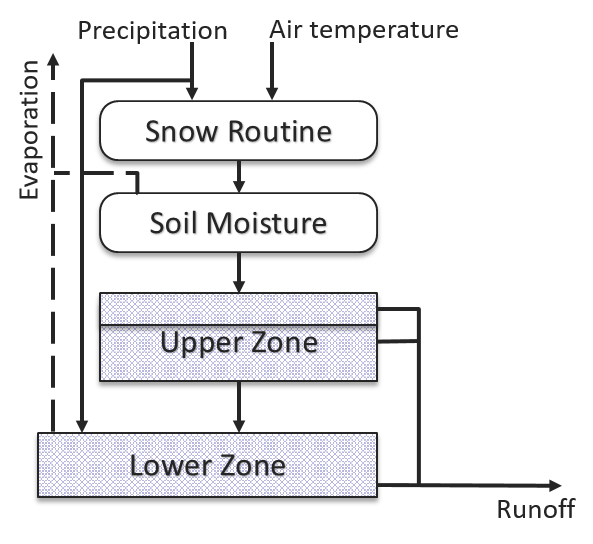
\includegraphics[width=0.6\textwidth]{fig/hydrology}
    \caption{Structure of the HBV model.}
    \label{fig:fig10}
\end{figure}

The model is developed for each water storage component to define the dynamics and balances of the water. In addition, the catchment area is divided into elevation zones (usually not more than ten) where each zone has the same area. The air temperature and the precipitation are provided for each elevation zone. Hence, all  calculations within each water storage component are performed for each elevation zone.

\subsubsection{Snow routine}

In the snow routine segment, the snow storage, as well as snowmelt are computed. This computation is performed for each elevation zone. Using the mass balance, the change in the dry snow storage volume $V_\mathrm{s,d}$, is found as follows:
\begin{equation}\label{eq:eq20}
\frac{dV_\mathrm{s,d}}{dt}=\dot{V}_\mathrm{p,s}-\dot{V}_\mathrm{d2w}
\end{equation}
Here, the flow of the precipitation in the form of snow is denoted as $\dot{V}_\mathrm{p,s}$. This precipitation in the form of snow is defined from the input precipitation flow, $\dot{V}_\mathrm{p}$, based on the information about the air temperature, $T$, a threshold temperature for snowmelt, $T_\mathrm{T}$, and for the area that is not covered by lakes (the fractional area covered by the lakes, $a_\mathrm{L}$, is used):
\begin{equation}\label{eq:eq21}
\dot{V}_\mathrm{p,s}=\begin{cases} \dot{V}_\mathrm{p}K_\mathrm{CR}K_\mathrm{CS}(1 - a_\mathrm{L}), & \mbox{if } T\leq T_\mathrm{T}\\ 0, & \mbox{if } T>T_\mathrm{T} \end{cases}
\end{equation}
Precipitation correction coefficients $K_\mathrm{CR}$ and $K_\mathrm{CS}$ are also used here, for the rainfall and snowfall precipitations, respectively. Then, the flow of precipitation in the form of rain is defined as follows:
\begin{equation}\label{eq:eq22}
\dot{V}_\mathrm{p,r}=\begin{cases} \dot{V}_\mathrm{p}K_\mathrm{CR}(1 - a_\mathrm{L}), & \mbox{if } T>T_\mathrm{T}\\ 0, & \mbox{if } T\leq T_\mathrm{T} \end{cases}
\end{equation}
The flow of the melting snow (melting of snow from dry form to water form), $\dot{V}_\mathrm{d2w}$, can be found using the following expression based on the degree-day factor $K_\mathrm{dd}$ and the area of the elevation zone $A_\mathrm{e}$:
\begin{equation}\label{eq:eq23}
\dot{V}_\mathrm{d2w}=\begin{cases} A_\mathrm{e}K_\mathrm{dd}(T - T_\mathrm{T})(1 - a_\mathrm{L}), & \mbox{if }T>T_\mathrm{T}\mbox{ and }V_\mathrm{s,d}>0\\ 0, & \mbox{otherwise} \end{cases}
\end{equation}
Finally, the flow out of the snow routine to the next soil moisture segment, $\dot{V}_\mathrm{s2s}$, is found as a sum of flows of precipitation in the form of rain, and the melted snow:
\begin{equation}\label{eq:eq24}
\dot{V}_\mathrm{s2s}=\dot{V}_\mathrm{p,r}+\dot{V}_\mathrm{d2w}
\end{equation}
It should be noted that a simplification related to the threshold temperature, $T_\mathrm{T}$, is assumed here. This threshold temperature describes both the snow melt and the rainfall to snowfall transition temperatures in the presented model. In reality, this threshold temperature might differ for each of these processes. In addition, the storage of snow in water form is not considered here, mostly due to the simplification with the threshold temperature.

\subsubsection{Soil moisture routine}

In the soil moisture segment, the water storage in the ground (soil) is found together with actual evapotranspiration from the snow-free areas. The net runoff to the next segment (upper zone) is also defined here. Using the mass balance, the volume of the soil moisture storage, $V_\mathrm{s,m}$, is found as follows:
\begin{equation}\label{eq:eq25}
\frac{dV_\mathrm{s,m}}{dt}=\dot{V}_\mathrm{s2s}-\dot{V}_\mathrm{s2u}-\alpha_\mathrm{e}\dot{V}_\mathrm{s,e}
\end{equation}
Here, $\dot{V}_\mathrm{s2u}$ is the net runoff to the next segment (the upper zone). $\dot{V}_\mathrm{s,e}$ is the actual evapotranspiration from the soil, that is taken into account only for the snow-free areas (zones). To define these snow-free zones, coefficient $\alpha_\mathrm{e}$ is used and equals one for snow-free areas and zero for covered-by-snow areas. The actual evapotranspiration can be found from the potential evapotranspiration, $\dot{V}_\mathrm{e}$, the volume of the soil moisture storage, $V_\mathrm{s,m}$, the area of the elevation zone $A_\mathrm{e}$, and the field capacity --- threshold soil (ground) moisture storage, $g_\mathrm{T}$:
\begin{equation}\label{eq:eq26}
\dot{V}_\mathrm{s,e}=\begin{cases} \frac{V_\mathrm{s,m}}{A_\mathrm{e}g_\mathrm{T}}\dot{V}_\mathrm{e}, & \mbox{if } V_\mathrm{s,m}< A_\mathrm{e}g_\mathrm{T}\\ \dot{V}_\mathrm{e}, & \mbox{if } V_\mathrm{s,m}\geq A_\mathrm{e}g_\mathrm{T} \end{cases}
\end{equation}
The potential evapotranspiration, $\dot{V}_\mathrm{e}$, is defined as the input to the hydrology model, similarly to the air temperature and precipitations.

The output of the soil moisture segment --- the net runoff to the next segment, $\dot{V}_\mathrm{s2u}$, can be found based on the field capacity, $g_\mathrm{T}$, as follows:
\begin{equation}\label{eq:eq27}
\dot{V}_\mathrm{s2u}=\begin{cases} \Big(\frac{V_\mathrm{s,m}}{A_\mathrm{e}g_\mathrm{T}}\Big)^{\beta}\dot{V}_\mathrm{s2s}, & \mbox{if } 0\leq V_\mathrm{s,m}< A_\mathrm{e}g_\mathrm{T}\\ \dot{V}_\mathrm{s2s}, & \mbox{if } V_\mathrm{s,m}\geq A_\mathrm{e}g_\mathrm{T} \end{cases}
\end{equation}
Here, $\beta$ is an empirical parameter for specifying the relationship between the flow out of the snow routine, the soil moisture storage, and the net runoff from the soil moisture. Typically,  $\beta \in [2,3]$, which leads to nonlinearity in Eq.~\ref{eq:eq27}.

\subsubsection{Runoff routine}

The upper and lower zones from Figure~\ref{fig:fig10} are combined into one segment --- the runoff routine. In this segment, the runoff from the catchment area is found based on the outflow from the soil moisture. The effects of the precipitation to, and evapotranspiration from the lakes in the catchment area are also taken into account here.

The upper zone characterises components with quick runoff. The following mass balance is used for the upper zone description:
\begin{equation}\label{eq:eq28}
\frac{dV_\mathrm{u,w}}{dt}=\dot{V}_\mathrm{s2u}-\dot{V}_\mathrm{u2l}-\dot{V}_\mathrm{u2s}-\dot{V}_\mathrm{u2q}
\end{equation}
Here, $V_\mathrm{u,w}$ is the water volume in the upper zone that depends on the saturation threshold, $s_\mathrm{T}$, which defines the surface (fast) runoff, $\dot{V}_\mathrm{u2s}$, and the fast runoff, $\dot{V}_\mathrm{u2q}$. $\dot{V}_\mathrm{u2b}$ is the runoff to the lower zone and is defined by the percolation capacity, $K_\mathrm{PC}$, for the area that is not covered by lakes:
\begin{equation}\label{eq:eq29}
\dot{V}_\mathrm{u2l}=A_\mathrm{e}(1-a_\mathrm{L})K_\mathrm{PC}
\end{equation}
The surface runoff, $\dot{V}_\mathrm{u2s}$, can be found using the saturation threshold, $s_\mathrm{T}$, and the water volume in the upper zone, $V_\mathrm{u,w}$:
\begin{equation}\label{eq:eq30}
\dot{V}_\mathrm{u2s}=\begin{cases} a_1(V_\mathrm{u,w}-A_\mathrm{e}s_\mathrm{T}), & \mbox{if } V_\mathrm{u,w}>A_\mathrm{e}s_\mathrm{T}\\ 0, & \mbox{if } V_\mathrm{u,w}\leq A_\mathrm{e}s_\mathrm{T} \end{cases}
\end{equation}
Here, $a_1$ is a parameter that represents the recession constant for the surface runoff. A similar recession constant, $a_2$, is used for the fast runoff, $\dot{V}_\mathrm{u2q}$, calculations:
\begin{equation}\label{eq:eq31}
\dot{V}_\mathrm{u2q}=a_2\min{(V_\mathrm{u,w},A_\mathrm{e}s_\mathrm{T})}
\end{equation}
The lower zone characterises the lake and the groundwater storages and defines the base runoff from the catchment area. The following mass balance equation is used for the lower zone description:
\begin{equation}\label{eq:eq32}
\frac{dV_\mathrm{l,w}}{dt}=\dot{V}_\mathrm{u2l}+a_\mathrm{L}\dot{V}_\mathrm{p}-\dot{V}_\mathrm{l2b}-a_\mathrm{L}\dot{V}_\mathrm{e}
\end{equation}
The water volume in the lower zone is denoted as $V_\mathrm{l,w}$. As mentioned previously, $\dot{V}_\mathrm{p}$ and $\dot{V}_\mathrm{e}$ are the precipitation and the potential evapotranspiration flows, respectively. $a_\mathrm{L}$ is the fractional area covered by lakes. $\dot{V}_\mathrm{l2b}$ is the base runoff from the lower zone that can be found as follows:
\begin{equation}\label{eq:eq33}
\dot{V}_\mathrm{l2b}=a_3V_\mathrm{l,w}
\end{equation}
Here, $a_3$ is the recession constant similar to $a_1$ and $a_2$.

The total runoff from the catchment, $\dot{V}_\mathrm{tot}$, is a sum of the base, quick, surface runoffs for each elevation zones, and is defined as follows:
\begin{equation}\label{eq:eq34}
\dot{V}_\mathrm{tot}=\sum\limits_{i=1}^n(\dot{V}_{\mathrm{l2b},i}+\dot{V}_{\mathrm{u2s},i}+\dot{V}_{\mathrm{u2q},i})
\end{equation}
Here, the base $\dot{V}_{\mathrm{l2b},i}$, quick $\dot{V}_{\mathrm{u2q},i}$, and surface $\dot{V}_{\mathrm{u2s},i}$ runoffs are first summed up for each of the $n$ elevation zones and then these sums of the base, quick and surface runoffs are added together.

Hence, this hydrology model is encoded in the \emph{OpenHPL} library as the \emph{RunOff\_zones} unit where the main defined variable is the total runoff from the catchment. This unit uses the standard Modelica connector \emph{RealOutput} connector as an output from the model that can be connected to, for example, simple reservoir model \emph{Reservoir} unit.

In order to get historic information about the air temperature, precipitation, and potential evapotranspiration for each of the elevation zones, the standard Modelica \emph{CombiTimeTable} source models are used in order to read this data from the text files.

When the \emph{RunOff\_zones} unit is in use, the user can specify the required geometry parameters for the catchment: the number of elevation zones, all hydrology parameters such as threshold temperatures, degree-day factor, precipitation correction coefficients, field capacity and $\beta$ parameter in soil moisture routine, threshold level for quick runoff in upper zone, percolation from upper zone to lower zone, recession constants for the surface and quick runoffs in upper zone, and recession constant for the base runoff in lower zone. Finally, the user can also specify the info about the text files where the data for the \emph{CombiTimeTable} models are stored.

\section{Electro-Mechanical}

\subsection{Turbine}

The turbine unit can be expressed with a simple turbine model based on a look-up table (turbine efficiency vs. guide vane opening). This simple turbine model is described by Eq.~\ref{eq:eq35}, \cite{LieL:18,Vyt:19b}, where the mechanical turbine shaft power $\dot{W}_\mathrm{tr}$ is defined as:

\begin{equation}\label{eq:eq35}
\dot{W}_\mathrm{tr} = \eta_\mathrm{h}\Delta p_\mathrm{tr}\dot{V}_\mathrm{tr}
\end{equation}

Here, $\eta_\mathrm{h}$ gives the turbine hydraulic efficiency that is found from a standard turbine look-up table and depends on the turbine control signal, $u_v$. $\Delta p_\mathrm{tr}$ is the pressure drop through the turbine that is defined as the difference between inlet and outlet turbine pressures, i.e., $\Delta p_\mathrm{tr} = p_\mathrm{tr1}-p_\mathrm{tr2}$. The relationship between the turbine volumetric flow rate $\dot{V}_\mathrm{tr}$ and the pressure drop $\Delta p_\mathrm{tr}$ is described through a simple valve-like expression as follows:

\begin{equation}\label{eq:eq36}
\dot{V}_\mathrm{tr} = C_\mathrm{v} u_\mathrm{v} \sqrt{\frac{\Delta p_\mathrm{tr}}{p^\mathrm{a}}}
\end{equation}

Here, $C_\mathrm{v}$ in Eq.~\ref{eq:eq36} is some guide vane ``valve capacity'' that can be tuned by using the nominal turbine net head (nominal pressure drop) and the nominal turbine flow rate. $p^\mathrm{a}$ is the atmospheric pressure.

Based on Eqs.~\ref{eq:eq35} and \ref{eq:eq36}, the simple turbine model is implemented in \emph{OpenHPL} as the \emph{Turbine} element.  In this \emph{Turbine} unit, the multi-physic connections are used in order to stay connected to waterway units as well as to the other electro-mechanical units. Those connections are already implemented in the \emph{TurbineContacts} connectors model that is used in this \emph{Turbine} unit. Then, this unit can be connected to other waterway and electro-mechanical units.

In the \emph{Turbine} unit, the user can specify the required parameters for the simple turbine model:  guide vane ``valve capacity'' $C_\mathrm{v}$, the nominal turbine net head (nominal pressure drop) and the nominal turbine flow rate, turbine guide vane nominal opening signal  $u_{v,n}$ in per unit value from 0 to 1. The user can also choose either to use the constant turbine efficiency and specify it, or to use the look-up table for the turbine efficiency and also specify this table.

\subsection{Francis}

 Our library also includes a mechanistic Francis turbine model based on the Euler turbine equations. The key quantities of the model are shown in Fig.~\ref{fig:fig11}, and the shaft power $\dot{W}_s$ produced in the Francis turbine is defined as follows, \cite{LieL:18,Vyt:18}:

\begin{equation} \label{eq:eq37}
{\dot{W}_s} = \dot{m}\omega \Big(R_1\frac{\dot{V}}{A_1}\cot{\alpha_1}-R_2\big(\omega R_2+\frac{\dot{V}}{A_2}\cot{\beta_2}\big)\Big).
\end{equation}

\begin{figure}
\centering
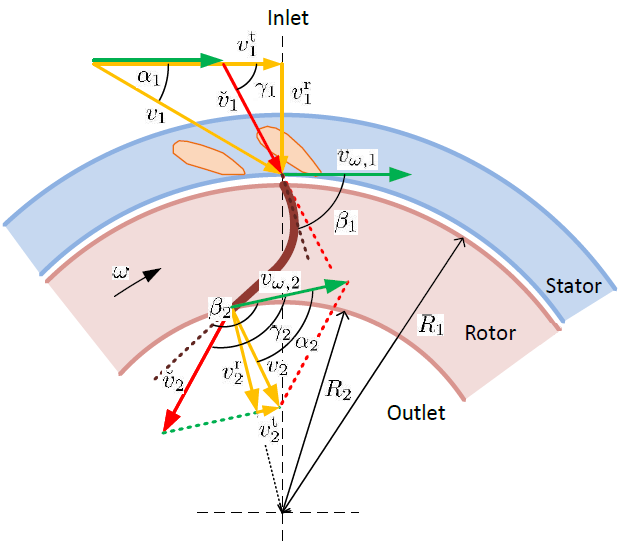
\includegraphics[width=0.6\textwidth]{fig/Fig_2_F_turb}    % The printed column width is 8.4 cm.
\caption{Key quantities in the Francis turbine model, with blade angles $\beta_1$ and $\beta_2$. The water effluent comes out from the paper plane, \cite{LieL:18}.}
\label{fig:fig11}
\end{figure}

Here, $\dot{m}$ and $\dot{V}$ are the mass and volumetric flow rate through the turbine, respectively, and $\omega$ is the angular velocity of the runner. $R_1$ and $R_2$ are the inlet and outlet radius of the runner, respectively. $A_1$ and $A_2$ are the inlet and outlet cross-sectional areas, respectively, and can be defined by using the runner dimensions: $R_1$, $R_2$, and $w_1$ which is the inlet width/height of the runner/blades. $\alpha_1$ is the inlet guide vane angle that is given by a control signal. $\beta_2$ is the outlet blade angle.

The total work rate $\dot{W}_t$ removed through the turbine is:

\begin{equation} \label{eq:eq38}
{\dot{W}_t} = {\dot{W}_s+\dot{W}_{ft}+\Delta p_v\dot{V}}.
\end{equation}

Here, $\Delta p_v$ is the pressure loss across the guide vane due to friction and is often neglected.
The total work rate might also be formulated based on Bernoulli's law: $\dot{W}_t=\Delta p_{tr}\dot{V} + \frac{1}{2}\dot{m}\dot{V}^2(\frac{1}{A_0^2}-\frac{1}{A_2^2})$, from where the total pressure loss across the turbine $\Delta p_{tr}$ can be defined; $A_0$ is the inlet cross section area to the spiral case. $\dot{W}_{ft}$ -- the friction term that represents various friction losses within the turbine is calculated as follows:

\begin{equation} \label{eq:eq39}
\begin{array}{ll}
\dot{W}_{ft} = k_{ft,1}\dot{V}(\cot{\gamma_1}-\cot{\beta_1})^2 \\
+k_{ft,2}\dot{V}\cot^2{\alpha_2}+k_{ft,3}\dot{V}^2.
\end{array}
\end{equation}

Here, $k_{ft,1}$, $k_{ft,2}$ and $k_{ft,3}$ are friction coefficients that represent shock, whirl, and pipe friction losses, respectively. These coefficients are tuning parameters for the mechanistic Francis turbine model. $\beta_1$ is the inlet blade angle which in the nominal operating condition should be equal to the angle of the relative velocity $\gamma_1$ in order to achieve an influent no-shock condition (the angle of the relative velocity is defined from: $\cot{\gamma_1}=\cot{\alpha_1}-\frac{\omega R_1}{\dot{V}}A_1$). To satisfy the no-whirl effluent condition, angle $\alpha_2$ should be equal to 0. This angle is defined as $\cot{\alpha_2}=\cot{\beta_2}+\frac{\omega R_2}{\dot{V}/A_2}$.

We propose the following expressions for the turbine loss coefficients, \cite{Vyt:19b}:
\begin{equation}
\begin{array}{c}
k_{ft,1} = 11.6\cdot10^3e^{8.9\cdot10^{-3}H_\mathrm{n}}\\
k_{ft,2} = 0\\
k_{ft,3} = 720e^{6.7\cdot10^{-3}H_\mathrm{n}}
\end{array}
\end{equation}

The efficiency of the turbine can be defined as follows:
\begin{equation} \label{eq:eq40}
{\eta} = \frac{\dot{W}_{s}}{\dot{W}_{t}}
\end{equation}

\textbf{Turbine design algorithm.} Geometry parameters for the Francis turbine must be found in order to use the mechanistic turbine model as presented above. These parameters, such as blade angles or runner dimensions, can be found from design data. Typically, for real (in use) turbines, these data are unavailable due to trade confidentiality. Thus, it is of interest to develop a design algorithm that can be used to define all the geometry parameters. The structure of this algorithm is shown in Fig.~\ref{fig:fig12}, where the input and output values for the design algorithm are presented.

\begin{figure}
\begin{center}
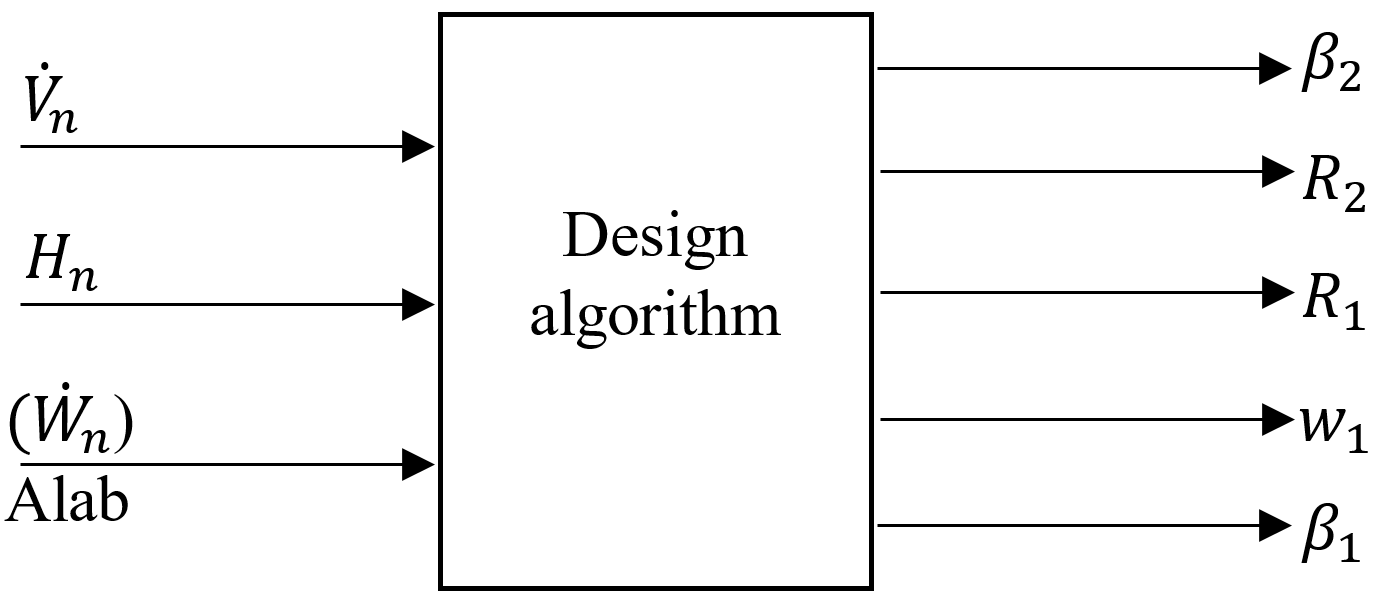
\includegraphics[width=0.4\textwidth]{fig/Fig_3_Algor_str} % The printed column width is 8.4 cm.
\caption{Block diagram that describes the turbine design algorithm (inputs and outputs).}
\label{fig:fig12}
\end{center}
\end{figure}

As input data for the calculation, nominal net head $H_n$ and volumetric flow rate $\dot{V}_n$ are used. A possible turbine design algorithm is as follows, ref. Fig.~\ref{fig:fig11}, \cite{Bre:01}:

\begin{enumerate}
  \item Choose the outlet blade angle $\beta_2$ and reference velocity $v_{\omega,2}$. These values are usually in the interval:
\begin{equation} \label{eq:eq41}
\begin{array}{ll}
158\mathrm{^\circ} \leq \beta_2 \leq 165\mathrm{^\circ} \\
35\mathrm{m/s} \leq v_{\omega,2} \leq 42\mathrm{m/s}
\end{array}
\end{equation}
  Here, the outlet angle and reference velocity take higher values for higher heads. Brekke suggests that these  values may be chosen as $\beta_2=162.5\mathrm{^\circ}$ and $v_{\omega,2}=41\mathrm{m/s}$.
  \item Define the outlet runner cross-section area $A_2$ (radius $R_2$) and adjust it together with reference velocity $v_{\omega,2}$ to the normal synchronous rotational speed.\\First, the meridional velocity is defined as:
\begin{equation} \label{eq:eq42}
{v_2^r} = -\frac{v_{\omega,2}}{\cot{\beta_2}},
\end{equation}
then outlet radius can be defined from the outlet cross-sectional area ($A_2=\pi R_2^2$):
\begin{equation} \label{eq:eq43}
{v_2^r} = \frac{\dot{V}}{A_2} \Rightarrow R_2=\sqrt{\frac{\dot{V}}{\pi v_2^r}}
\end{equation}
Then, the turbine rotational speed $n$ [$\mathrm{RPM}$] can be calculated from the angular velocity ($\omega=\frac{\pi n}{30}$):
\begin{equation} \label{eq:eq44}
{v_{\omega,2}}={\omega R_2} \Rightarrow n=\frac{30v_{\omega,2}}{\pi R_2}
\end{equation}
After this the turbine speed should be reduced to the nearest synchronous speed (depends on number of pole pairs $p$ in the generator: $n=\frac{60f}{p}$, where frequency $f$ is constant $50\,\mathrm{Hz}$) and then the outlet radius with the reference velocity should be recalculated in reverse order, using~(\ref{eq:eq44}),~(\ref{eq:eq43}) and~(\ref{eq:eq42}).\\ Normally, the information about the turbine rotational speed is available, so the outlet runner radius and the reference velocity can be found directly from~(\ref{eq:eq42}),~(\ref{eq:eq43}) and~(\ref{eq:eq44}).
  \item Choosing the inlet runner dimension, inlet cross-section area $A_1$ (radius $R_1$ and width $w_1$).\\ The inlet radius can be defined from the reference velocity $v_{\omega,1}$ as follows:
\begin{equation} \label{eq:eq45}
{R_1}=\frac{v_{\omega,1}}{\omega}=\frac{30v_{\omega,1}}{\pi n}
\end{equation}
Here, the reference velocity can be chosen from the range of reduced value $\overline{v}_{\omega,1}\in [0.7, 0.75]$, which is dimensionless and expressed as:
\begin{equation} \label{eq:eq46}
{\overline{v}_{\omega,1}} = \frac{v_{\omega,1}}{\sqrt{2gH}}
\end{equation}
It is common to use $\overline{v}_{\omega,1}=0.725$.\\Regularly, in order to avoid backflow in the runner, an acceleration of the flow through the runner is desirable. That is why the outlet meridional velocity can be chosen approximately ten per cent higher than the inlet.
\begin{equation} \label{eq:eq47}
{v_2^r} = 1.1v_1^r
\end{equation}
Then the inlet runner width $w_1$ can be calculated from the inlet cross-sectional area ($A_1=2\pi R_1w_1$):
\begin{equation} \label{eq:eq48}
{v_1^r} = \frac{\dot{V}}{A_1}\Rightarrow w_1=\frac{\dot{V}}{2\pi R_1v_1^r}
\end{equation}
Here, it should be noted that the blade thickness could be included for improving the calculation of the inlet cross-section area, e.g., 10\% of the perimeter.
  \item The inlet blade angle $\beta_1$ can be found as follows:
\begin{equation} \label{eq:eq49}
{\tan{(180^\circ-\beta_1)}} = \frac{v_1^r}{v_{\omega,1}-v_1^t}
\end{equation}
  Here, $v_1^t$ is the tangential velocity and can be defined from dimensionless value $\overline{v}_1^t = 0.48/\overline{v}_{\omega,1}$, using~(\ref{eq:eq46}) to convert from dimensionless value.
\end{enumerate}

\textbf{Guide vane actuation.} In addition, a model for the guide vane opening is also included in order to define the inlet guide vane angle $\alpha_1$, \cite{LieL:18}. The guide vane geometry is depicted in Figure~\ref{fig:fig13}.
\begin{figure}
\begin{center}
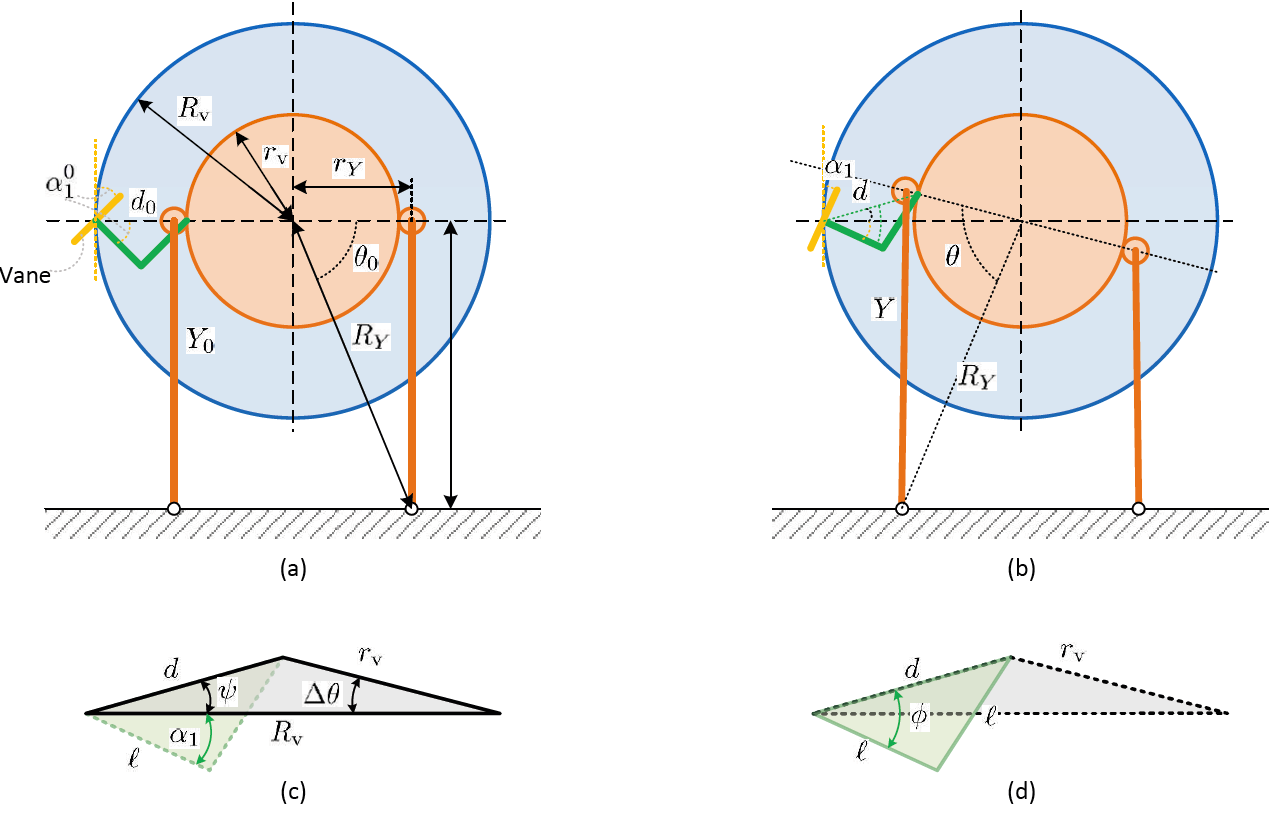
\includegraphics[width=0.8\textwidth]{fig/Guide_vane} % The printed column width is 8.4 cm.
\caption{Guide vane geometry relating actuator position $Y$ to guide vane angel $\alpha_1$, \cite{LieL:18}.}
\label{fig:fig13}
\end{center}
\end{figure}

From Figure~\ref{fig:fig13}~(a), assuming that the actuator cylinder is ``vertical'' in position ``0'', it can be found that
\begin{equation}
\begin{array}{c}
{R}_Y^2=r_Y^2+Y_0^2 \\
\cos\theta_0=\frac{r_Y}{R_Y}
\end{array}
\end{equation}

Clearly, $d_0=R_v-r_v$. Next, moving the actuator to position $Y$, Figure~\ref{fig:fig13}~(b) with the cosine law gives
\begin{equation}
Y^2=r_Y^2+R_Y^2-2r_YR_Y\cos\theta
\end{equation}
thus specifying angle $\theta$. The change in angel $\theta$ is introduced in (Figure~\ref{fig:fig12}~(b), (c)) as
\begin{equation}
\Delta\theta\equiv\theta-\theta_0
\end{equation}

Then, applying the cosine law to Figure~\ref{fig:fig13}~(c) gives length $d$ ($d\in[d_0,2l]$) from
\begin{equation}
d^2=r_v^2+R_v^2-2r_vR_v\cos\Delta\theta
\end{equation}
and then angle $\psi$ from
\begin{equation}
r_v^2=d^2+R_v^2-2dR_v\cos\psi
\end{equation}
Here, it is necessary to ensure that the sign of $\psi$ equals to the sign of $\Delta\theta$.

From Figure~\ref{fig:fig13}~(d) and applying the cosine law, we find
\begin{equation}
l^2=l^2+d^2-2ld\cos\phi\Rightarrow\cos\phi=\frac{d}{2l}
\end{equation}

Finally, the guide vane angle can be found as
\begin{equation}
\alpha_1=\phi-\psi
\end{equation}

In the above model, it has been assumed that the guide vane is perpendicular to the attached ``arm'' of length $l$, and that in position ``0'', a guide vane is at position ``9 o'clock'', Figure~\ref{fig:fig13}~(a), \cite{LieL:18}.

Hence, together the Francis turbine model, the turbine design algorithm and the guide vane actuation (servo position) are realized in the \emph{Francis} turbine element in our library.  In this \emph{Francis} unit, the multi-physic\emph{TurbineContacts} connectors model is also used and ensures connection to other waterway and electro-mechanical units. In addition, this \emph{Francis} unit has also the standard Modelica \emph{RealInput} connector that describes the angular velocity as an input to the Francis turbine model. Typically, this angular velocity connector is based on the derived info from (connected to) the generator units.

In the \emph{Francis} unit, the user can specify the required nominal parameters for the Francis turbine:  nominal turbine net head (nominal pressure drop), nominal turbine flow rate, nominal power, and nominal rotational speed. Then, the user can either choose to use the design algorithm that automatically defines the turbine geometry parameters (radius of the turbine blade inlet and outlet, the width of the turbine/blades inlet, the turbine inlet and outlet blade angles), or specify these turbine geometries manually. Similarly, the user has the same options for the losses coefficients and parameters for the guide vane actuation (servo position) model.

\subsection{Pelton}

Similar to the Francis turbine model, the mechanistic Pelton turbine model is developed and used. The key quantities of the model are shown in Fig.~\ref{fig:fig14}, and the shaft power $\dot{W}_s$ produced in the Pelton turbine is defined as follows, \cite{LieL:18}:
\begin{figure}
\begin{center}
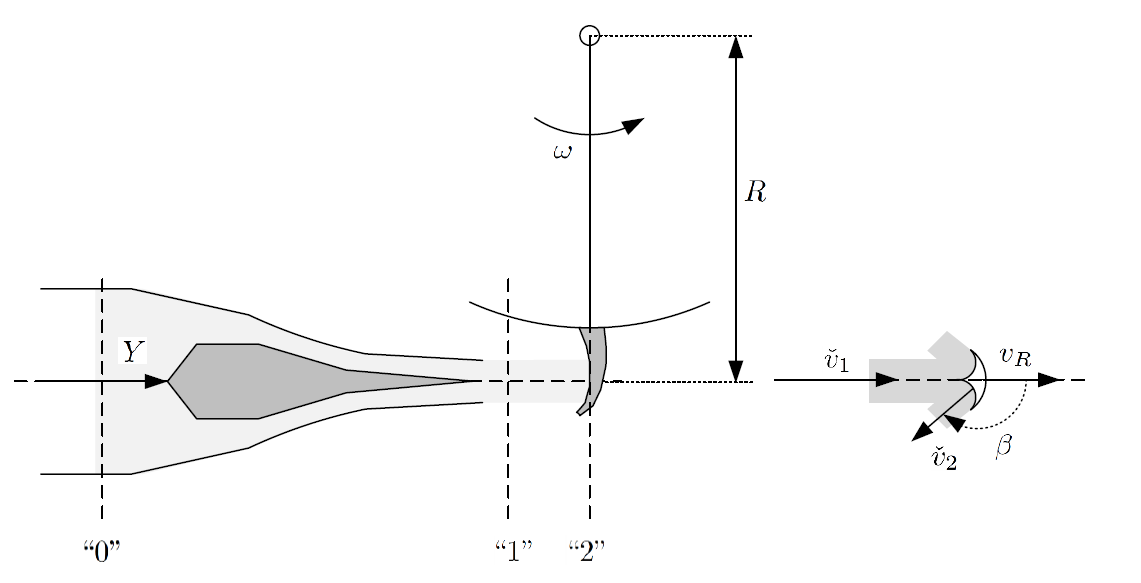
\includegraphics[width=0.8\textwidth]{fig/Pelton_turb} % The printed column width is 8.4 cm.
\caption{Some key concepts of the Pelton turbine, \cite{LieL:18}.}
\label{fig:fig14}
\end{center}
\end{figure}

\begin{equation}
\dot{W}_s=\dot{m}v_R\left[\delta(u_\delta)\cdot v_1-v_R\right]\left(1-k\cos\beta\right)
\end{equation}
Here, $\dot{m}$ is the mass flow rate through the turbine. The reference velocity is equal to $v_R = \omega R$: here, $R$ is a is the radius of the rotor where the mass hits the bucket and $\omega$ is the angular velocity that is normally constrained by the grid frequency. The water velocity at position ``1'' (Figure~\ref{fig:fig14}) is equal to $v_1=\frac{\dot{V}}{A_1}$, where $\dot{V}$ is the volumetric flow rate through the turbine and $A_1$ is a cross-sectional area at position ``1'' (the end of the nuzzle). $\beta$ is the reflection angle with typical value of $\beta= 165^{\circ}$, and $k<1$ is some friction factor, typically $k\in[0.8, 0.9]$, \cite{LieL:18}. In practical installations, there is a deflector mechanism to reduce the velocity $v_1\delta(u_\delta)$ to avoid over-speed.

The total work rate $\dot{W}_t$ removed through the turbine is:
\begin{equation} \label{eq:eq50}
{\dot{W}_t} = {\dot{W}_s+\dot{W}_{ft}}
\end{equation}
Here, $\dot{W}_{ft}$ is a friction of losses that can be found as follows:
\begin{equation}
\dot{W}_{ft}=K\left(1-k\cos\beta\right)\dot{m}v_R^2
\end{equation}
Here, friction coefficient $K$ equals 0.25, \cite{LieL:18}.

In addition, the pressure drop across the nozzle (positions ``0'' and ``1'`) $\Delta p_n$ can be found as follows, \cite{LieL:18}:
\begin{equation}
\Delta p_n=\frac{1}{2}\rho\dot{V}\left[\dot{V}\left(\frac{1}{A_1^2(Y)}-\frac{1}{A_0^2}\right)+k_f\right]
\end{equation}
Here, $A_0$ is a cross sectional area at position ``0'' (the beginning of the nuzzle). $A_1(Y)$ means that the cross-sectional area at position ``1'' is a function of the needle position $Y$. $k_f$ is a coefficient of friction loss in the nuzzle.

Hence, this Pelton turbine model is realized in the \emph{Pelton} turbine element in our library.  In this \emph{Pelton} unit, the multi-physic\emph{TurbineContacts} connectors model is also used and ensures connection to other waterway and electro-mechanical units. In addition, this \emph{Pelton} unit also has the standard Modelica \emph{RealInput} connector that describes the angular velocity as an input to the Francis turbine model. Typically, this angular velocity connector is based on the derived info from (connected to) the generator units.

In the \emph{Pelton} unit, the user can specify the required geometry for the Pelton turbine: radius of the turbine runner, input diameter of the nuzzle, runner bucket angle, friction factors and coefficients, and deflector mechanism coefficient.

\subsection{Simple Generator}

Here, a simple model of an ideal generator with friction is considered. This model has inputs as electric power available on the grid and the turbine shaft power. This model is based on the angular momentum balance which depends on the turbine shaft power, the friction loss in the aggregate rotation, and the power taken up by the generator. The rotor angular velocity mainly depends on its inertia, internal friction and available power. The kinetic energy stored in the rotating generator is $ K_a=\frac{1}{2}J_a\omega_a^2$, where $\omega_a$ is the angular velocity of the rotor and $J_a$ is its moment of inertia. The kinetic energy $K_a$ is changed by the power terms operating on the generator axis, e.g., the turbine shaft power $\dot{W}_s$ produced by the turbine, friction power $\dot{W}_{f,a}$, and the power taken up by the generator, $\dot{W}_g$, \cite{LieL:18}, and from energy the balance can be expressed as follows:
\begin{equation}
\frac{dK_a}{dt}=\dot{W}_s-\dot{W}_{f,a}-\dot{W}_g
\end{equation}
$\dot{W}_{f,a}$ is the frictional power loss in the rotor. This frictional power loss is mainly due to losses in the shaft supporting bearings, losses in the transmission gearboxes and losses in the windage (air gap). For simplicity, it is assumed that the bearing term is dominating, and express $\dot{W}_{f,a}$ as
\begin{equation}
\dot{W}_{f,a}=\frac{1}{2}k_{f,b}\omega_a^2
\end{equation}
Here, $k_{f,b}$ is the bearing friction factor. The power taken up by the generator is transmitted to the grid with electric efficiency $\eta_e$. Thus the electric power available on the grid is $\dot{W}_e=\eta_e\dot{W}_g$.

Hence, this simple generator model is encoded in the \emph{OpenHPL} as a \emph{SimpleGen} unit. This unit has inputs as electric power available on the grid and the turbine shaft power which both are implemented with the standard Modelica \emph{RealInput} connector. This \emph{SimpleGen} unit also uses the standard Modelica \emph{RealOutput} connectors in order to provide output information about the angular velocity and frequency of the generator. All these connectors can be connected to turbines units and other standard Modelica blocks.

In the \emph{SimpleGen} unit, the user can specify the required parameters for the generator: moment of inertia of the generator, generator's electrical efficiency, friction factor in the rotor bearing box, the number of the generator poles. This unit can be initialised by the initial value of the angular velocity $\omega_0$. Otherwise, the user can decide on an option when the simulation starts from a steady-state and the OpenModelica automatically handles the initial steady-state values (does not work properly in OpenModelica).

\subsection{Synchronize Generator}

Here, a more detailed model of the synchronous generator is presented. More details in the Behzad Sharefi master thesis, \cite{Sha:11}. This model is based on the d-q decomposition and assumed that the generator is connected to the grid, \cite{Sha:11}. The voltage-current relation is given as:
\begin{equation}
\left[\begin{matrix}R_a+R_e & x_q'+x_e\\ -x_d'-x_e & R_a+R_e\end{matrix}\right]\left[\begin{matrix}I_d \\ I_q\end{matrix}\right]= \left[\begin{matrix}E_d'+V_s\sin\delta_e \\ E_q'-V_s\cos\delta_e\end{matrix}\right]
\end{equation}
Here, $R_a$ and $R_e$ are the phase winding and equivalent network resistances, $x_d$, $x_q$, $x_d'$, and $x_q'$ are d-/q-axis normal, and transient reactances. $x_e$ is the equivalent network reactance. $I_d$ and $I_q$ are the d-/q-axis currents. $E_d'$ and $E_q'$ are the d-/q-axis transient voltages. $V_s$ is the network RMS (Root-Mean-Squared) voltage. $\delta_e$ is the phase shift angle that is described as follows:
\begin{equation}
\frac{d\delta_e}{dt} = (\omega - \omega_s)\frac{n_p}{2}
\end{equation}
Here, $n_p$ is the number of poles in the generator, where $\omega$ and $\omega_s$ are the generator and grid angular velocities, respectively. The Swing equation is used to describe the angular velocity dynamics and looks as follows:
\begin{equation}
\frac{d\omega}{dt}=\frac{\dot{W}_s-P_e}{J\omega}
\end{equation}

The dynamic equations for the transient operation are as follows:  \begin{equation}
\begin{array}{c}
T_{qo}'\frac{dE_d'}{dt} =-E_d' + (x_q' - x_q)I_q \\
T_{do}'\frac{dE_q'}{dt} = -E_q' + (x_d - x_d')I_d + E_f
\end{array}
\end{equation}
Here, $T_{do}'$ and $T_{qo}'$ are the d-/q-axis transient open-circuit time constants. $E_f$ is the voltage across the field winding with the following dynamic equation:
\begin{equation}
\frac{dE_f}{dt} = \frac{-E_f + K_E\left(V_{tr}-V_t-V_{stab}\right)}{T_E}
\end{equation}
Here, $K_E$ is the excitation system gain and $T_E$ --- excitation system time constant. $V_{tr}$ is the voltage reference set point for the exciter.
$V_t$ is the terminal voltage and can be found as $V_t = \sqrt{\left(E_d'-R_aI_d-x_q'I_q\right)^2+\left(E_q'-R_aI_q+x_d'I_d\right)^2}$. $V_{stab}$ is the stabilisation voltage with the following dynamic equation:
\begin{equation}
\frac{dV_{stab}}{dt} = \frac{-V_{stab} + K_F\frac{dE_f}{dt}}{T_{FE}}
\end{equation}
Here, $K_F$ is the stabiliser gain, and $T_{FE}$ --- the stabiliser time constant.

The output active and reactive power of the generator can be found as follows:
\begin{equation}
\begin{array}{c}
P_e = 3\left(E_d'I_d+E_q'I_q\right)\\
Q_e = \sqrt{9V_t^2I_t^2-P_e^2}
\end{array}
\end{equation}
Here, the terminate current is given as $I_t=\sqrt{I_d^2+I_q^2}$.

Hence, this synchronise generator model is encoded in the \emph{OpenHPL} as a\emph{SynchGen} unit. This unit has inputs as the turbine shaft power, that is implemented with the standard Modelica \emph{RealInput} connector. This \emph{SynchGen} unit also uses the standard Modelica \emph{RealOutput} connectors in order to provide output information about the angular velocity and frequency of the generator. All these connectors can be connected to turbines units and other standard Modelica blocks.

In the \emph{SynchGen} unit, the user can specify the required nominal parameters for the generator: active and reactive powers drawn from the generator at Steady-State operating condition, phase winding resistance, and the number of poles. The following network parameters should be also specified by the user: equivalent network resistance and reactance, network RMS voltage, grid angular velocity. The user also specifies the d-/q-axis normal and transient reactances, d-/q-axis transient open-circuit time constants, minimum and maximum field voltages, excitation system, stabilizer gains, time constants, moment of inertia of the generator, and the friction factor in the rotor bearing box. This unit can be initialized, or the user can decide on an option for the self initialisation.

\section{Governor}

Here, a simple model of the governor that controls the guide vane opening in the turbine based on the reference power production is described. More details in the Behzad Sharefi master thesis, \cite{Sha:11}. The block diagram of this governor model is shown in Figure~\ref{fig:fig15}.
\begin{figure}
\begin{center}
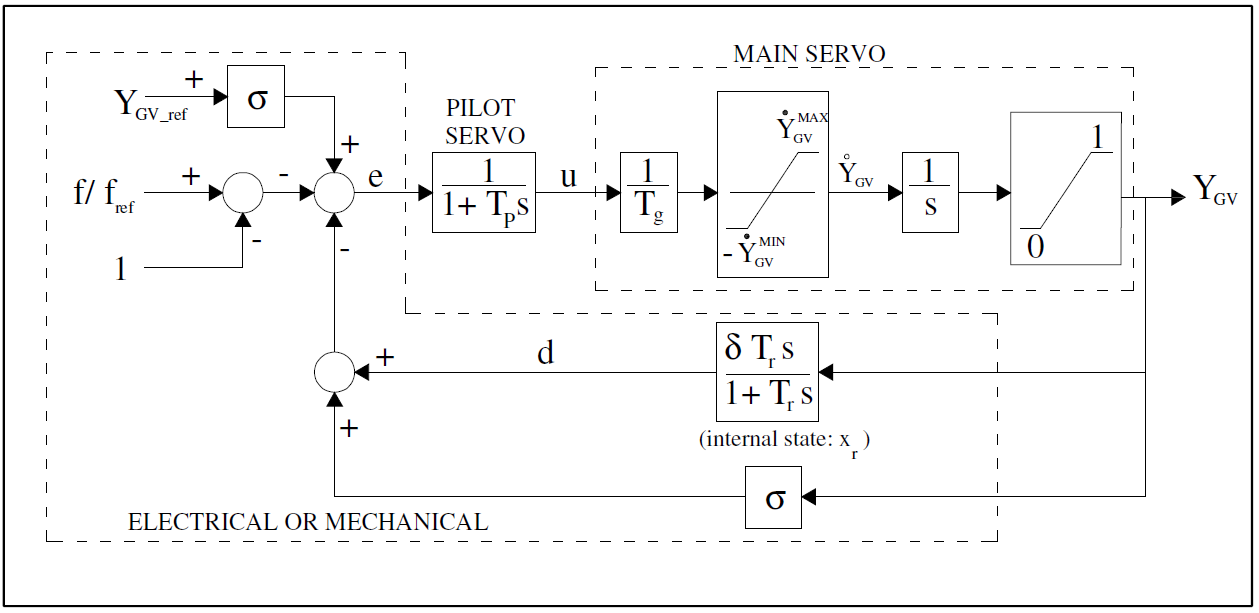
\includegraphics[width=0.8\textwidth]{fig/Governor} % The printed column width is 8.4 cm.
\caption{Block Diagram of the governor, \cite{Sha:11}.}
\label{fig:fig15}
\end{center}
\end{figure}

Using the model in Figure~\ref{fig:fig15} and the standard Modelica blocks, the governor model is encoded in our library as the \emph{Governor} unit. This unit has inputs as the reference power production and generator frequency that are implemented with the standard Modelica \emph{RealInput} connector. This \emph{Governor} unit also uses the standard Modelica \emph{RealOutput} connectors in order to provide output information about the turbine guide vane opening.

In the \emph{SynchGen} unit, the user can specify the various time constants of this model (see Figure~\ref{fig:fig15}): pilot servomotor time constant $T_p$, primary servomotor integration time $T_g$, and transient droop time constant $T_r$. The user should also provide the following parameters: droop value $\sigma$, transient droop $\delta$, and nominal values for the frequency and power generation. The information about the maximum, minimum, and initial guide vane opening should also be specified.

\section{Examples}

Here, various models that have been assembled in the \emph{Examples} class are described.

\subsection{HPSimple}

In this model of the hydropower system, the simplified models are used for conduits and turbine modelling. The generator is not included in the model. The simple \emph{Pipe} unit is used to represent the penstock, intake and discharge races. The simple \emph{Turbine} unit is used to represent the turbine. The \emph{Reservoir} unit is used to represent the reservoir and the tailwater (here, this unit uses a simple model of the reservoir that only depends on the water depth in the reservoir). Data from the Sundsbarm hydropower plant is used for this example model.

\subsection{HPSimple\_generator}

In this model of the hydropower system, the simplified models are used for conduits, turbine, and generator modelling. The simple \emph{Pipe} unit is used to represent the penstock, intake and discharge races. The simple \emph{Turbine} unit is used to represent the turbine. The \emph{SimpleGen} unit is used to represent the generator. The \emph{Reservoir} unit is used to represent the reservoir and tailwater (here, this unit uses a simple model of the reservoir that only depends on the water depth in the reservoir). Data from the Sundsbarm hydropower plant is used for this example model.

\subsection{HPSimple\_Francis}

In this model of the hydropower system, the simplified model is used for conduits modelling. The turbine and the generator are modelled with more detailed \emph{Francis} and \emph{SynchGen} units, respectively. The simple \emph{Pipe} unit is used to represent the penstock, intake and discharge races. The \emph{Reservoir} unit is used to represent the reservoir and the tailwater (here, this unit uses a simple model of the reservoir that only depends on the water depth in the reservoir). Data from the Sundsbarm hydropower plant is used for this example model.

\subsection{HPDetailed}

In this model of the hydropower system, the simplified models are used for conduits and turbine modelling, except for the penstock that is modelled with the more detailed \emph{PenstockKP} unit. The generator is not included in the model. The simple \emph{Pipe} unit is used to represent the intake and discharge races. The simple \emph{Turbine} unit is used to represent the turbine. The \emph{Reservoir} unit is used to represent the reservoir and the tailwater (here, this unit uses a simple model of the reservoir that only depends on the water depth in the reservoir). Data from the Sundsbarm hydropower plant is used for this example model.

\subsection{HPDetailed\_generator}

In this model of the hydropower system, the simplified models are used for conduits, turbine, and generator modelling, except for the penstock that is modelled with the more detailed \emph{PenstockKP} unit. The simple \emph{Pipe} unit is used to represent the intake and discharge races. The simple \emph{Turbine} unit is used to represent the turbine. The \emph{SimpleGen} unit is used to represent the generator. The \emph{Reservoir} unit is used to represent the reservoir and the tailwater (here, this unit uses a simple model of the reservoir that only depends on the water depth in the reservoir). Data from the Sundsbarm hydropower plant is used for this example model.

\subsection{HPDetailed\_Francis}

In this model of the hydropower system, the simplified model is used for conduits modelling, except for the penstock that is modelled with the more detailed \emph{PenstockKP} unit. The turbine and generator are modelled with more detailed \emph{Francis} and \emph{SynchGen} units, respectively. The simple \emph{Pipe} unit is used to represent the intake and discharge races. The \emph{Reservoir} unit is used to represent the reservoir and the tailwater (here, this unit uses a simple model of the reservoir that only depends on the water depth in the reservoir). Data from the Sundsbarm hydropower plant is used for this example model.

\subsection{HPSimple\_Francis\_IPSLGen}

Here, the last example model (uses the \emph{PenstockKP} and \emph{Francis} units) is extended by synergy with the \emph{OpenIPSL} for generator and power system modelling. The \emph{Governor} unit from the \emph{OpenHPL} is also used here. The penstock is modelled with the more detailed \emph{PenstockKP} unit. The turbine is modelled with more detailed \emph{Francis} unit. The simple \emph{Pipe} unit is used to represent the intake and discharge races. The \emph{Reservoir} unit is used to represent the reservoir and the tailwater (here, this unit uses a simple model of the reservoir that only depends on the water depth in the reservoir).

\subsection{HPSimple\_Francis\_GridGen}

Here, the \emph{HPDetailed\_Francis} example model (uses the \emph{PenstockKP} and \emph{Francis} units) is also extended by synergy with the \emph{OpenIPSL} for only generator modelling. The \emph{Governor} unit from the \emph{OpenHPL} is also used here. The penstock is modelled with the more detailed \emph{PenstockKP} unit. The turbine is modelled with the more detailed \emph{Francis} unit. The simple \emph{Pipe} unit is used to represent the intake and discharge races. The \emph{Reservoir} unit is used to represent the reservoir and the tailwater (here, this unit uses a simple model of the reservoir that only depends on the water depth in the reservoir).

\subsection{HPSimple\_Francis\_IPSLGenGov}

Here, the \emph{HPDetailed\_Francis} example model (uses the \emph{PenstockKP} and \emph{Francis} units) is extended by synergy with the \emph{OpenIPSL} for generator, governor and power system modelling. The penstock is modelled with the more detailed \emph{PenstockKP} unit. The turbine is modelled with the more detailed \emph{Francis} unit. The simple \emph{Pipe} unit is used to represent the intake and discharge races. The \emph{Reservoir} unit is used to represent the reservoir and the tailwater  (here, this unit uses a simple model of the reservoir that only depends on the water depth in the reservoir).

\subsection{HPSimple\_Francis\_IPSLGenInfBus}

Here, the \emph{HPDetailed\_Francis} example model (uses the \emph{PenstockKP} and \emph{Francis} units) is extended by synergy with the \emph{OpenIPSL} for generator and power system (including infinite bus) modelling. The \emph{Governor} unit from the \emph{OpenHPL} is also used here. The penstock is modelled with the more detailed \emph{PenstockKP} unit. The turbine is modelled with the more detailed \emph{Francis} unit. The simple \emph{Pipe} unit is used to represent the intake and discharge races. The \emph{Reservoir} unit is used to represent the reservoir and the tailwater  (here, this unit uses a simple model of the reservoir that only depends on the water depth in the reservoir).

\subsection{HPSimple\_OpenChannel}

In this model of the hydropower system, the simplified models are used for conduits and turbine modelling. The generator is not included in the model. The simple \emph{Pipe} unit is used to represent the penstock and intake race. The discharge race is an open channel here, and the \emph{OpenChannel} unit is used for modelling. The simple \emph{Turbine} unit is used to represent the turbine. The \emph{Reservoir} unit is used to represent the reservoir and the tailwater  (here, this unit uses a simple model of the reservoir that only depends on the water depth in the reservoir).

\chapter{Basic example}

Here, a basic (step-by-step) example is provided in order to show how to connect and specify elements from the \emph{OpenHPL} in a flowsheet. Furthermore, an example of how to set up the OMPython API is also presented.

\section{Flowsheet}

In order to create a flowsheet model for the hydropower system in OpenModelica using the \emph{OpenHPL}, the following steps should be performed:

\begin{enumerate}
    \item Create a new Modelica class that is specified as ``Model'' and assign a name for this model. Then, open this model with the ``Diagram view''. See example in Figure~\ref{fig:fig16}.
    \begin{figure}[ht]
    \begin{center}
    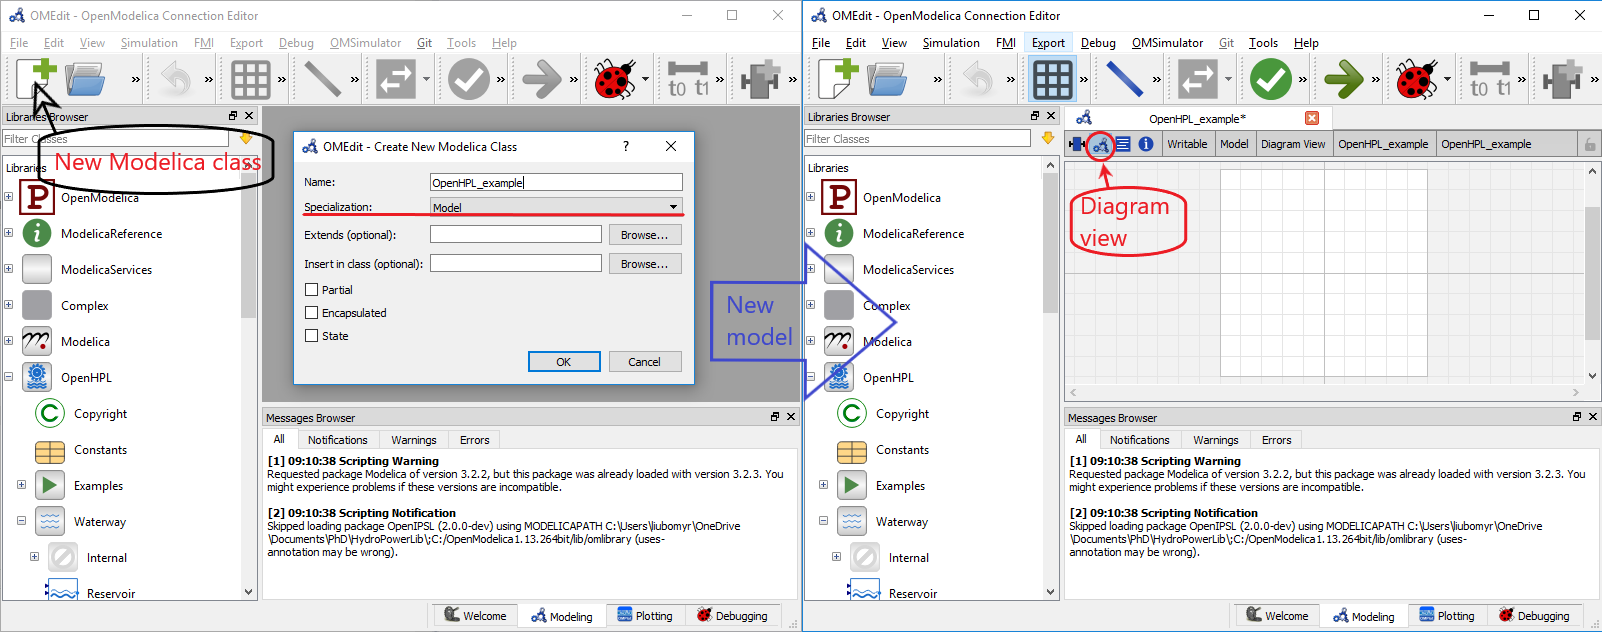
\includegraphics[width=1\textwidth]{fig/Exam_1} % The printed column width is 8.4 cm.
    \caption{Creating a new model in OpenModelica.}
    \label{fig:fig16}
    \end{center}
    \end{figure}
    \item Drag and drop all of the needed elements for the hydropower structure from the \emph{OpenHPL} and provide a name for each element. Then, connect the connectors of these elements between each other. See example in Figure~\ref{fig:fig17}.
    \begin{figure}
    \begin{center}
    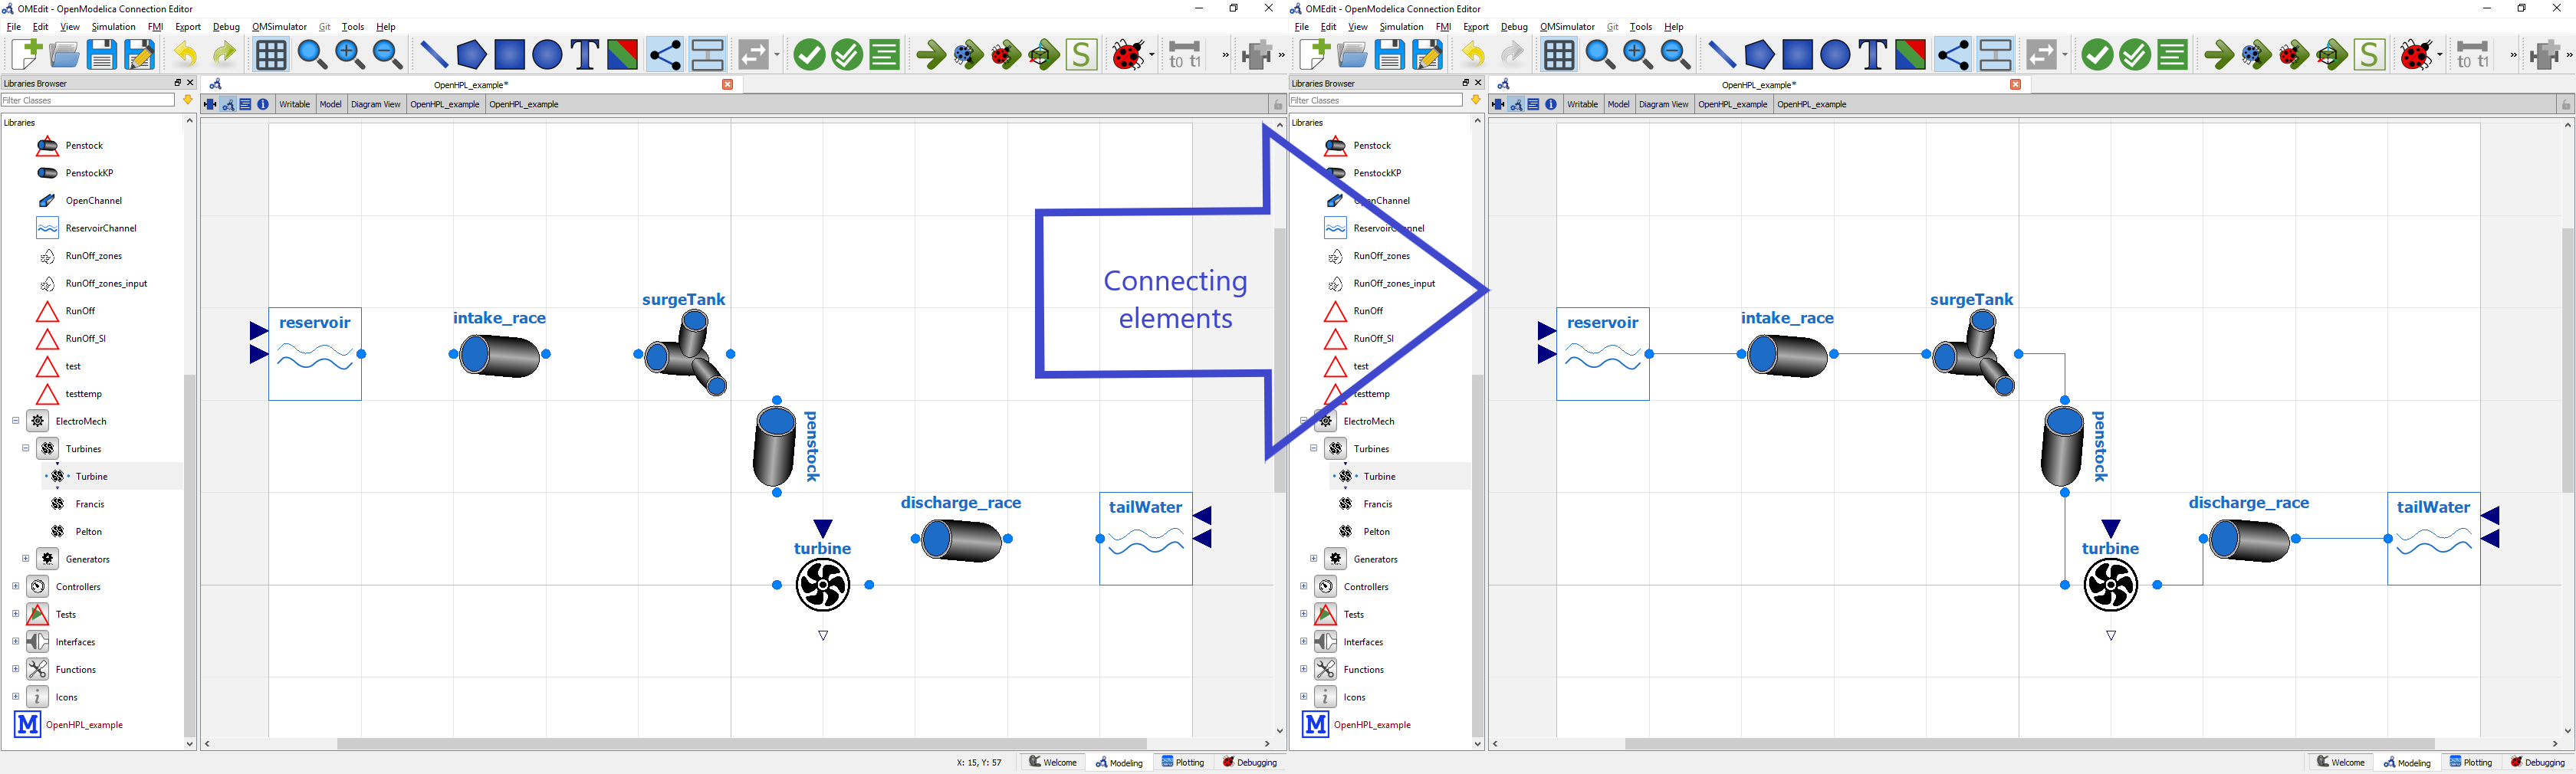
\includegraphics[width=1\textwidth]{fig/Exam_2} % The printed column width is 8.4 cm.
    \caption{Connecting the elements of the hydropower system.}
    \label{fig:fig17}
    \end{center}
    \end{figure}
    \item Also, insert the records model ``Constants'' from the \emph{OpenHPL} with the name ``Const'' to the model in order to have control on some constants and properties that are common for all hydropower elements. As an example in case, typical initial value of the volumetric flow rate in the system for each ``Pipe'' unit can be specified.
    \item Specify each of the elements with an appropriate geometry. See example for the specification of the intake race element in Figure~\ref{fig:fig18}.
    \begin{figure}[ht]
    \begin{center}
    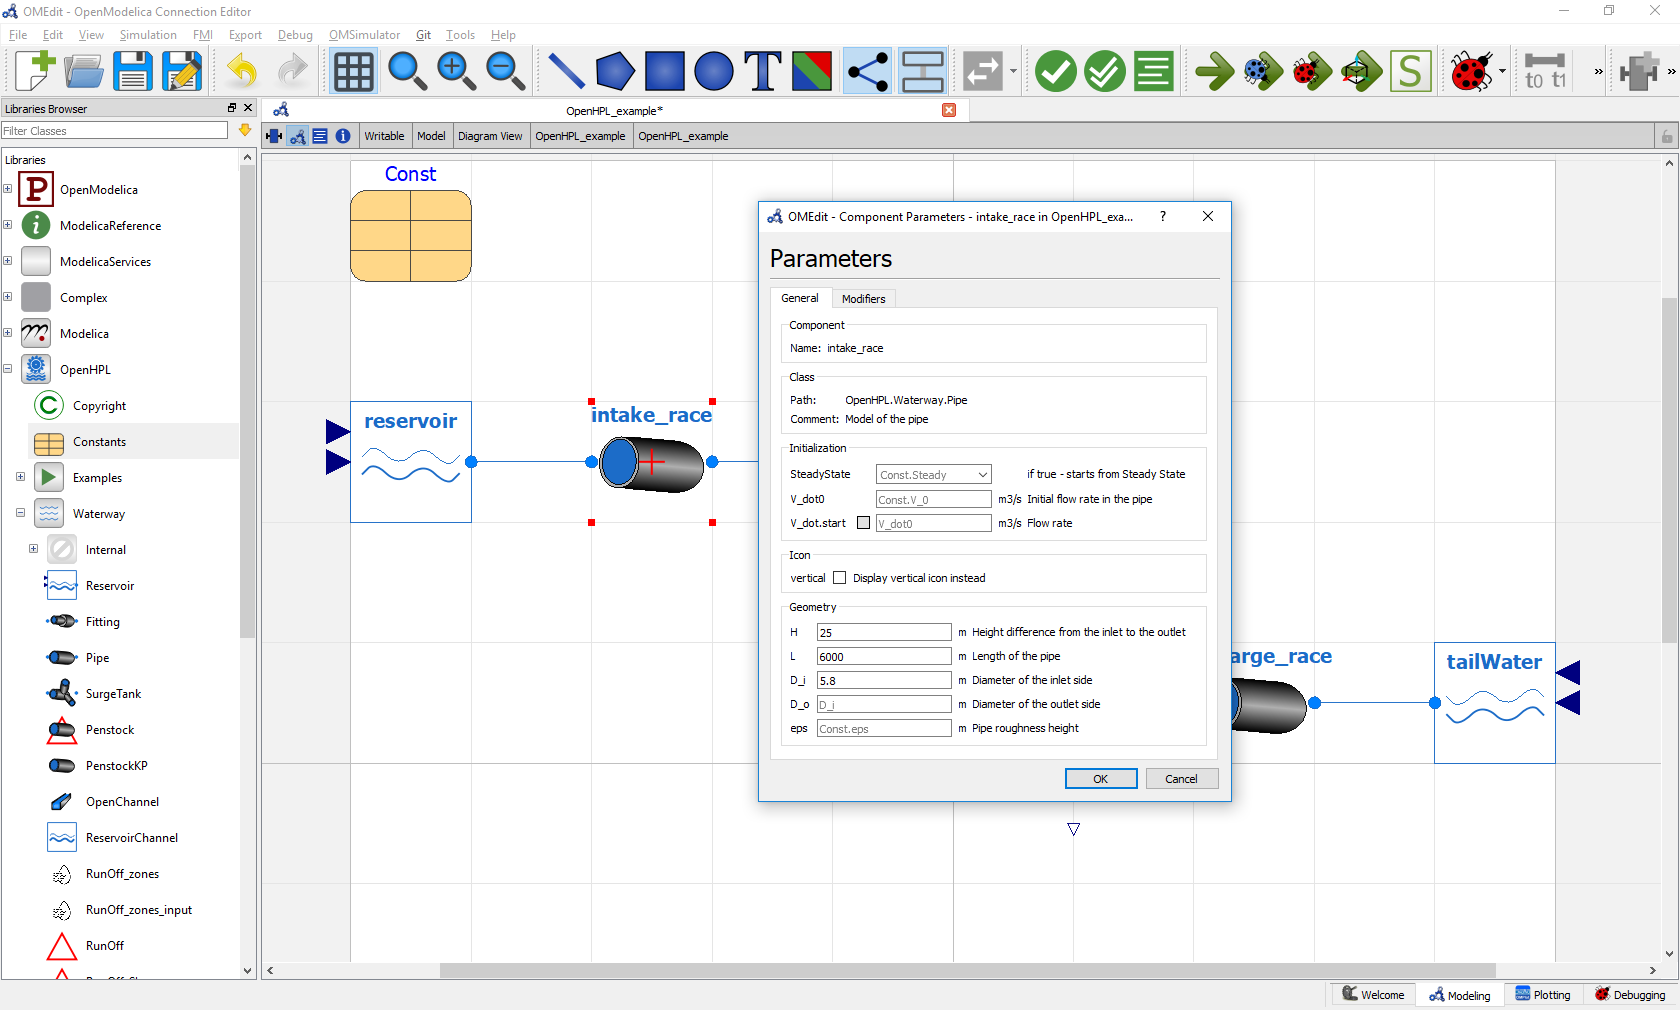
\includegraphics[width=0.8\textwidth]{fig/Exam_4} % The printed column width is 8.4 cm.
    \caption{Specification of the elements.}
    \label{fig:fig18}
    \end{center}
    \end{figure}
    \item Provide a control signal for the turbine. To make this, you can either add a source of the ramp signal from the standard Modelica library (``Modelica.Blocks.Sources. Ramp''), or create an input variable (or just a simple variable) for the example model ``OpenHPL example'' and equate it to the turbine control input. Both possibilities are shown in Figure~\ref{fig:fig19}.\label{example_control}
    \begin{figure}
    \begin{center}
    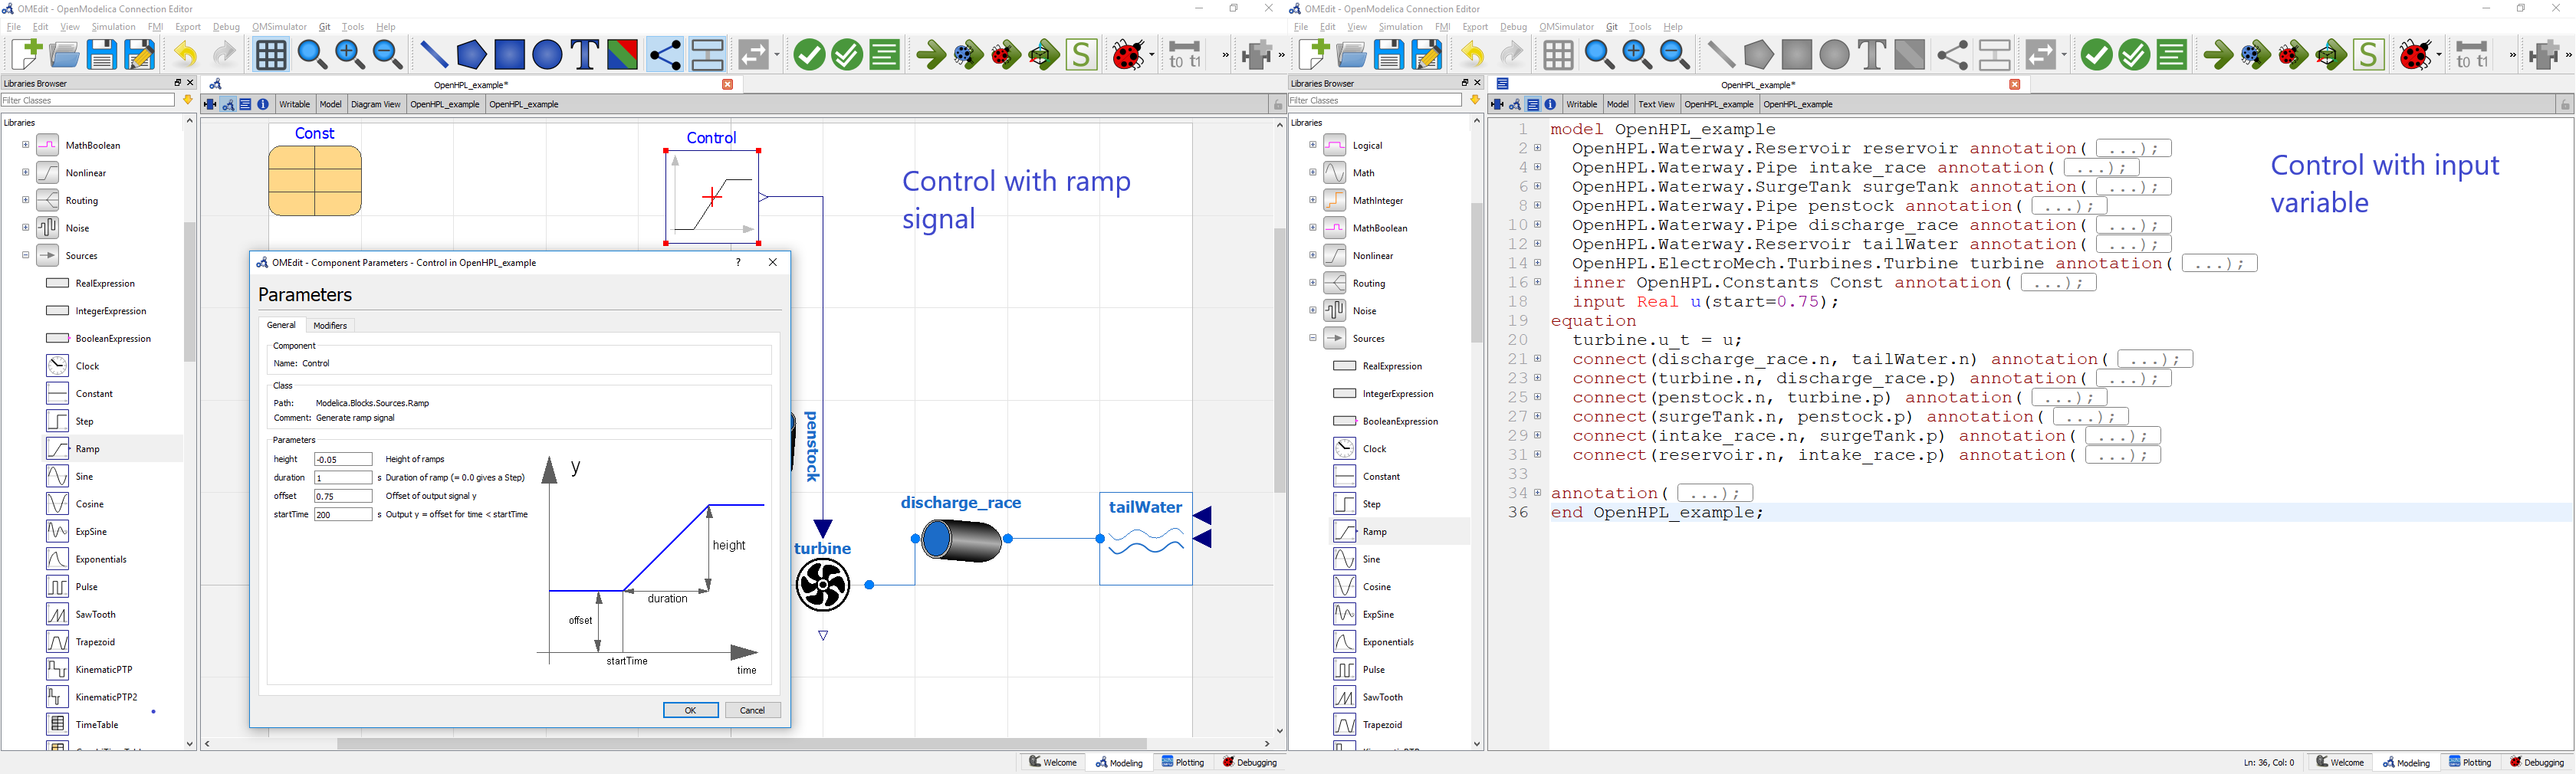
\includegraphics[width=1\textwidth]{fig/Exam_5} % The printed column width is 8.4 cm.
    \caption{Creating a control signal for the turbine.}
    \label{fig:fig19}
    \end{center}
    \end{figure}
    \item Specify the simulation setup values and save it in the model. Then, the simulation can be carried out. See example for the simulation specification and running in Figure~\ref{fig:fig20}.
    \begin{figure}[ht]
    \begin{center}
    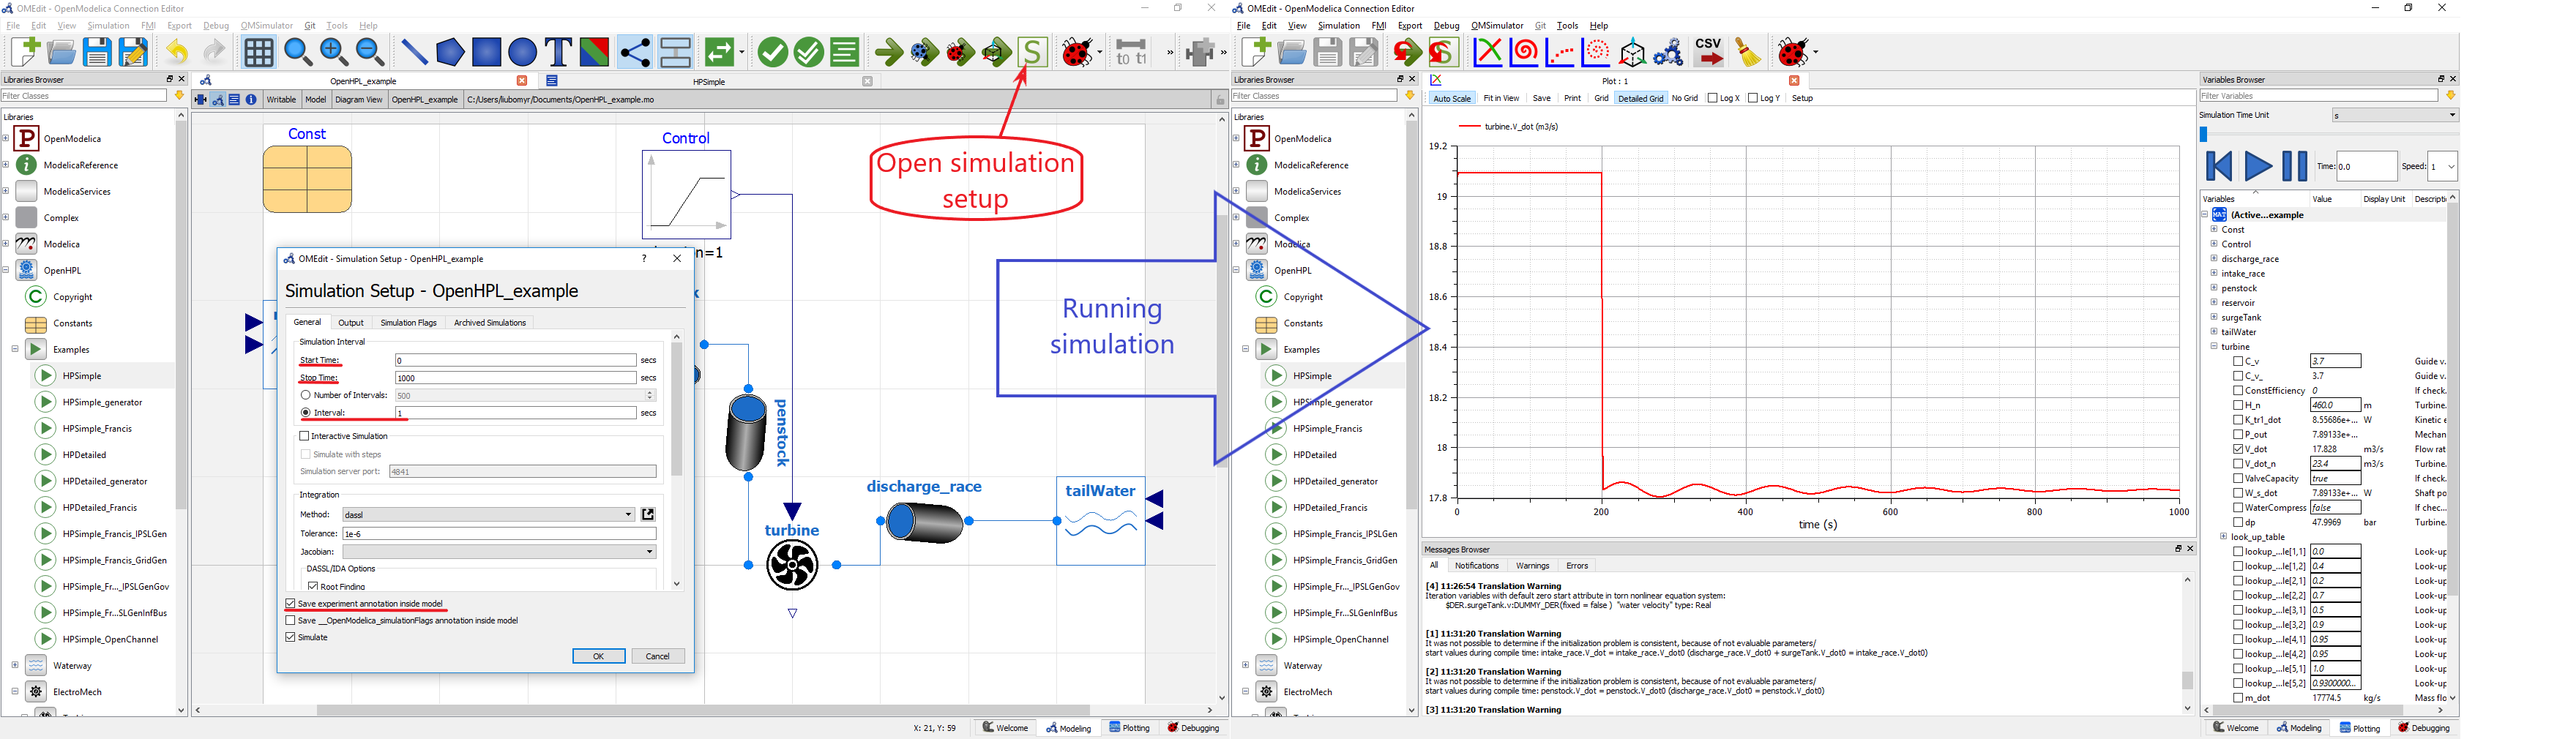
\includegraphics[width=1\textwidth]{fig/Exam_6} % The printed column width is 8.4 cm.
    \caption{Specifying and running simulation.}
    \label{fig:fig20}
    \end{center}
    \end{figure}
\end{enumerate}

\section{OMPython API}

In order to run the simulations of the developed example hydropower model from Python, the OMPython API for OpenModelica can be used. The following steps should be performed to set up the API:

\begin{enumerate}
    \item Import the ``Modelica system'' environment form the OMPython package. Then, create an object in Python of the OpenModelica model ``OpenHPL example''. Here, the libraries that are used in the model should also be loaded to the object which in this case, is the standard Modelica library and the \emph{OpenHPL}. See an example of the code below:
    \begin{lstlisting}[language = Python]
    from OMPython import ModelicaSystem
    hps_s = ModelicaSystem("OpenHPL_example.mo", "OpenHPL_example", ["Modelica", "OpenHPL/package.mo"])
    \end{lstlisting}
    \item When the object is created, the simulation options, as well as the parameters and input variables can be specified. In order to check and specify the simulation options, the following commands can be used:
    \begin{lstlisting}[language = Python]
    hps_s.setSimulationOptions(stepSize=0.1, stopTime=1000) # set simulation options
    hps_s.getSimulationOptions() # get list of simulation options
    \end{lstlisting}
    Similar commands for parameters and input variables look as follows:
    \begin{lstlisting}[language = Python]
    hps_s.getParameters() # get list of model parameters
    hps_s.setParameters(**{"turbine.H_n":460}) # set parameter value for the turbine nominal head
    hps_s.getInputs() # get list of input variables
    hps_s.setInputs(u=[(0,0.75),(100,0.75),(101,0.7),(1000,0.7)]) # set input value over time as a ramp signal
    \end{lstlisting}
    It should be noted that here, I used the model with input variable for the control signal of the turbine (see item \#\ref{example_control} and Figure~\ref{fig:fig19} in the previous flowsheet section).
    \item Run the simulation and get the results. An example of these commands are carried out as follows:
    \begin{lstlisting}[language = Python]
    hps_s.simulate() # run simulation
    hps_s.getSolutions() # get list of solution variables
    time, Vdot, p_tr1, p_tr2 = hps_s.getSolutions("time", "turbine.V_dot", "turbine.p_tr1", "turbine.p_tr2") # get results of simulation time variable, and the turbine flow rate, inlet and outlet pressures.
    \end{lstlisting}
    These simulation results can be then plotted using \emph{matplotlib} package. See the plots of the turbine flow rate and the pressures in Figure~\ref{fig:fig21}.
    \begin{figure}[ht]
    \begin{center}
    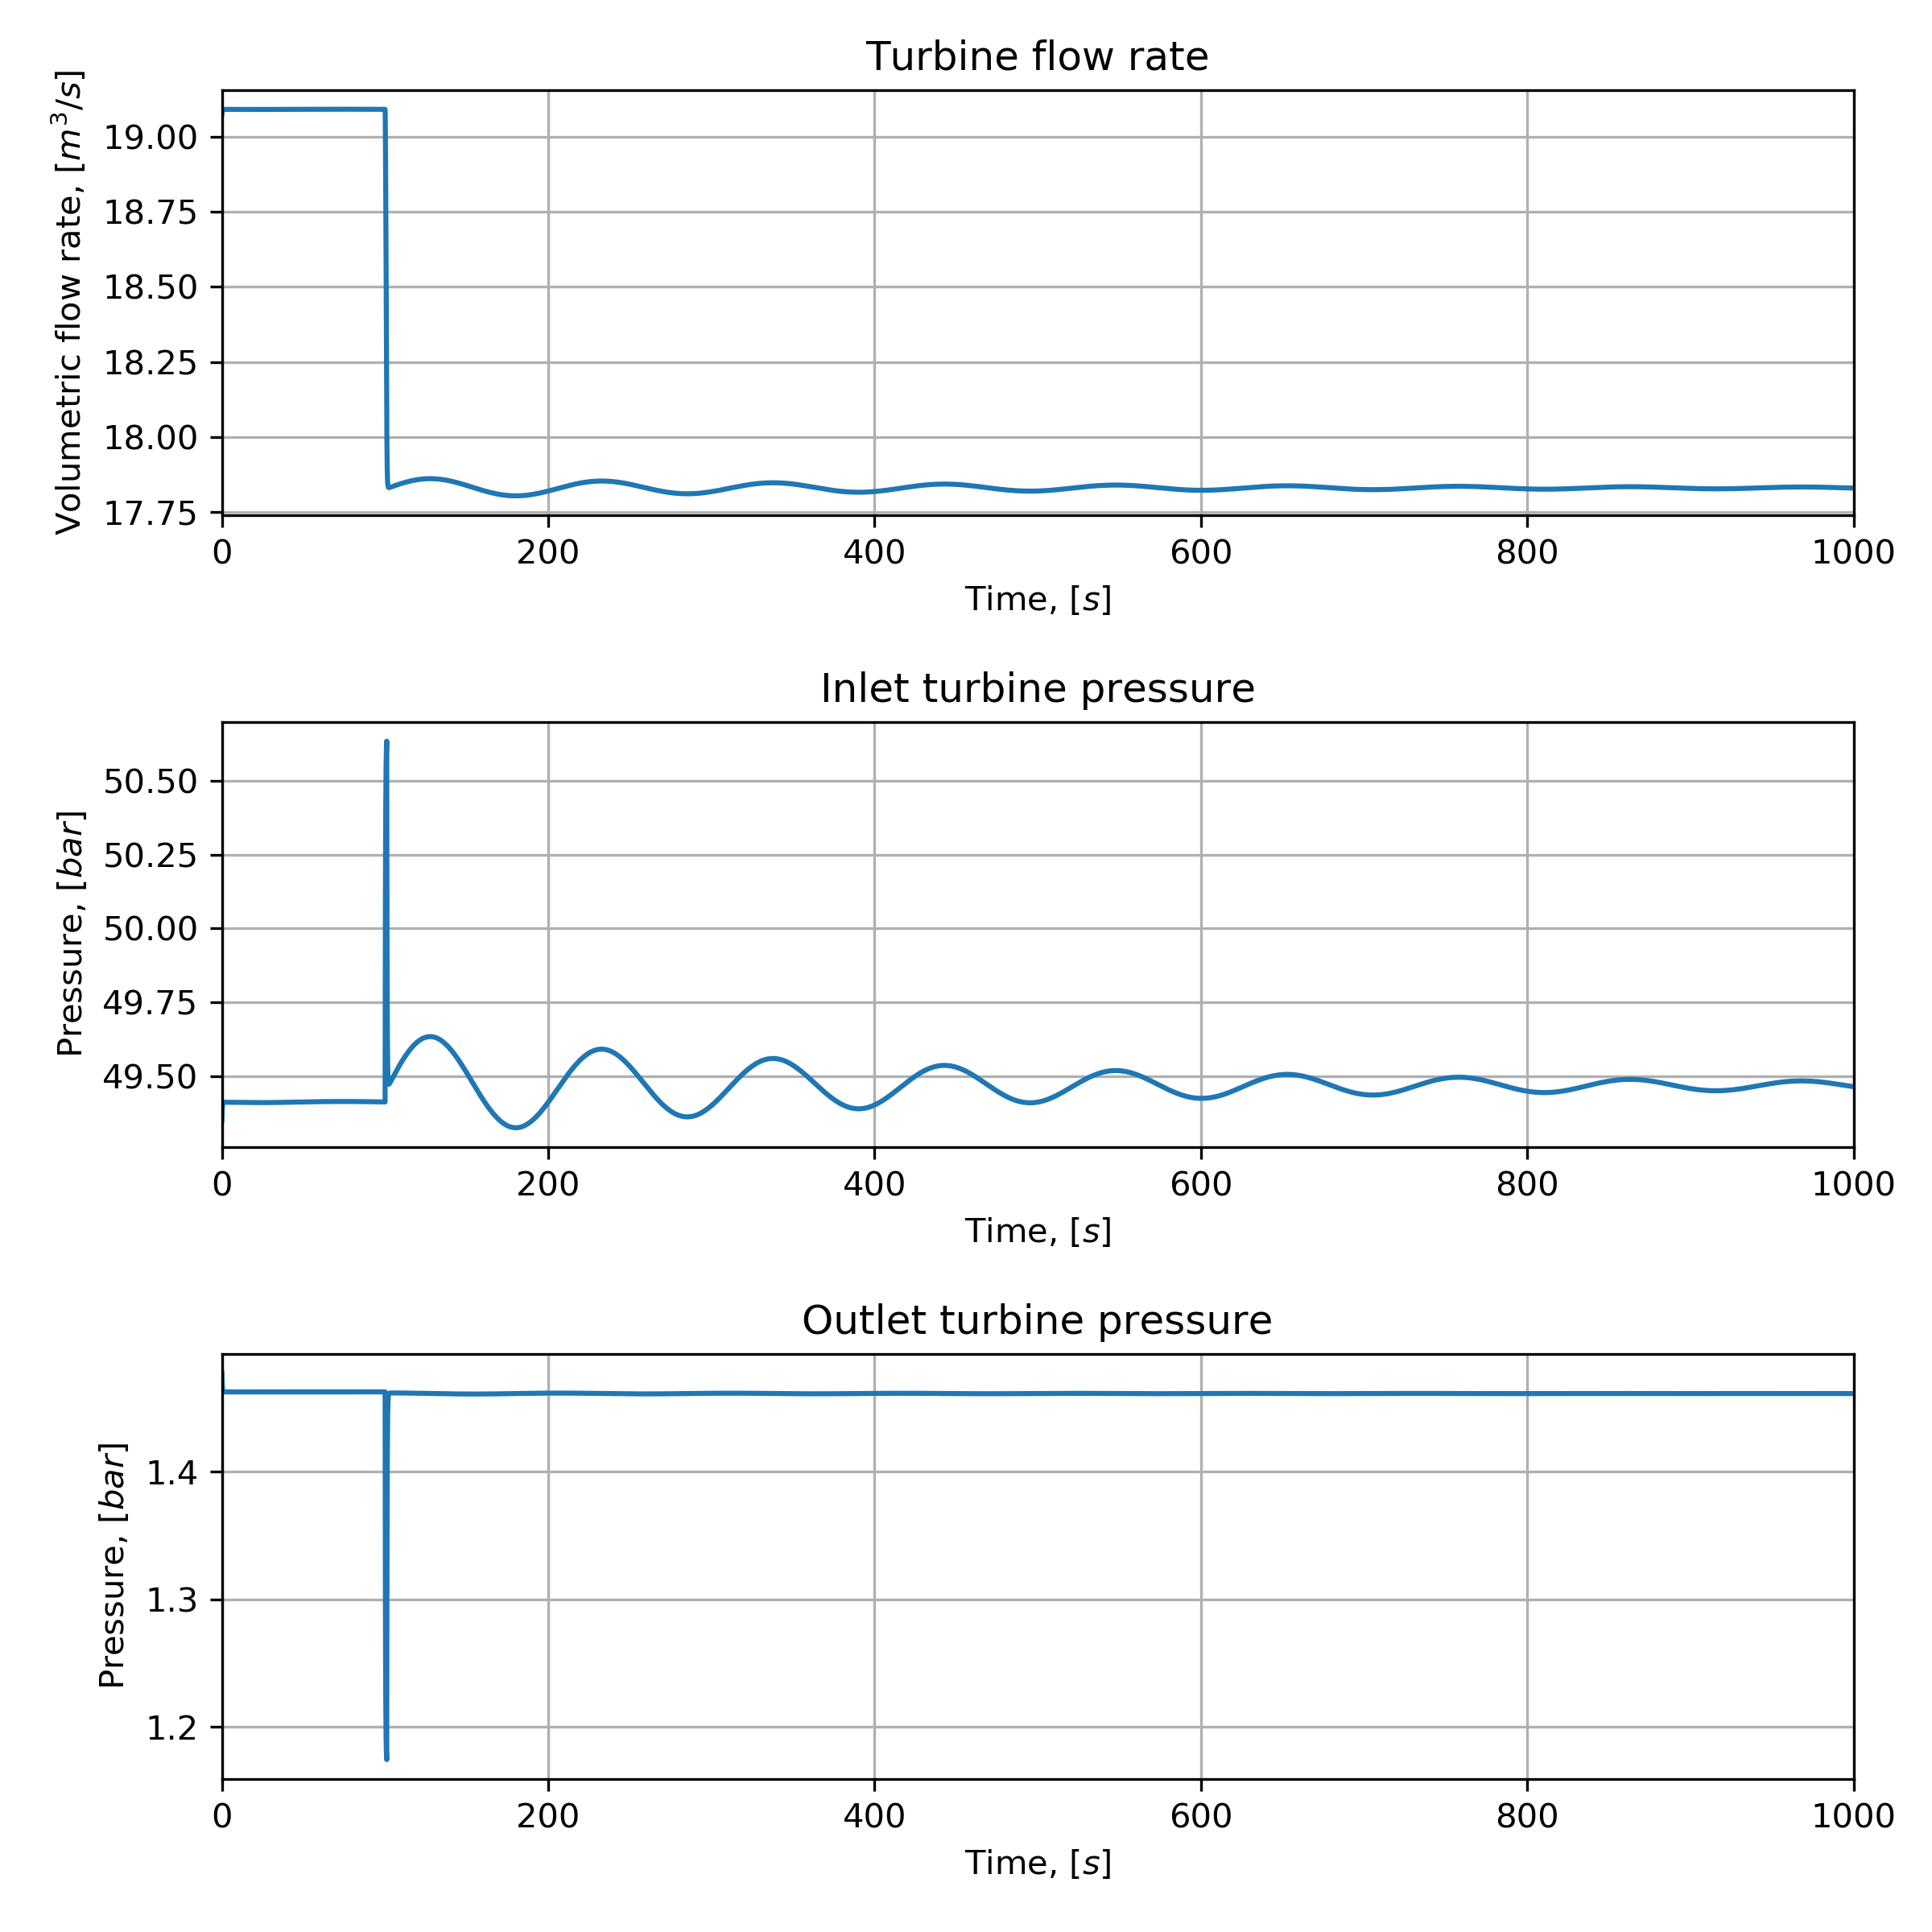
\includegraphics[width=0.7\textwidth]{fig/Exam_sim} % The printed column width is 8.4 cm.
    \caption{Plotting of simulation results.}
    \label{fig:fig21}
    \end{center}
    \end{figure}
    \item It is also possible to linearize the model for the future analysis. The linearization can be done with one command. However more commands can also be used to check/specify the linearization options and define the states/inputs/outputs. See the example below:
    \begin{lstlisting}[language = Python]
    hps_s.setLinearizationOptions(stopTime=0.1) # set a stop time for linearization (linearization is performed in this point)
    hps_s.getLinearizationOptions() # get a list of the linearization options
    As,Bs,Cs,Ds = hps_s.linearize() # actual linearization; defining standard A, B, C and D matrices.
    hps_s.getLinearStates() # get list of states
    hps_s.getLinearInputs() # get list of inputs
    hps_s.getLinearOutputs() # get list of outputs
    \end{lstlisting}
    It should be noted that the linearized model should include the input variable which in this case is the input variable for the turbine control signal.
\end{enumerate}

Similar to OMPython API, the running of OpenModelica models in Julia using OMJulia API can also be carried out. See the documentation of OMJulia for more information.

\cleardoublepage

% The bibliography should be displayed here...
\printbibliography[heading=bibintoc]
% You rather like to call the bibliography "References"? Then use this instead:
%\printbibliography[heading=bibintoc, title={References}]

\end{document}

%%% Local Variables:
%%% mode: latex
%%% TeX-master: t
%%% End:
